\section{State Estimation of 3D motion using Kalman Filters}
\subsection{Motion and Observation models}
\begin{enumerate}
\item 
We run the Kalman update after every $\Delta t$ timestep. The state $X_t \in \re^6$ denotes
\begin{align*}
X_t = \begin{bmatrix} x_t \\ y_t \\ z_t \\ \dot{x}_t \\ \dot{y}_t \\ \dot{z}_t \end{bmatrix}\\
\end{align*}
\item The initial belief $X_0 \sim \normal(0, 10^{-4} I_6)$ and $u_t = -10$ is a scalar. The motion model is
\begin{align*}
X_{t + 1} &= A_t X_{t} + B_t u_t + \epsilon_t\\
\text{where }
A_t &= \begin{bmatrix} 
I_3  & \Delta t \cdot I_3 \\ 
O_3 & I_3 \\ 
\end{bmatrix}
\text{, }
B_t = \begin{bmatrix} 
0 \\
0 \\
\frac{1}{2} \Delta t^2 \\
0 \\
0 \\
\Delta t 
\end{bmatrix}
\text{, }
\epsilon_t \sim \normal(0, R_t)\\
\text{where }
R_t &= \text{diag}(\sigma_x^2, \sigma_y^2, \sigma_z^2, \sigma_{\dot{x}}^2, \sigma_{\dot{y}}^2, \sigma_{\dot{z}}^2)
\end{align*}
\item The observations from IMU sensor are noisy  values of ball's position and velocity.

\item The observations from GPS sensor are noisy  values of ball's position.

\item The observations from BS sensor are noisy  values of ball's distances from $(32, -50, 10), (-32, -50, 10), (-32, 50, 10), (32, 50, 10)$ respectively. 

\item See observation models in \autoref{tab:obs_model}.
\end{enumerate}.

\begin{table}[H]
    \centering
    \begin{tabular}{|c|c|c|c|c|}
        \hline
        Sensor & $z_t$ & $Z_t$ & $C_t$ & $Q_t$ \\
        \hline
        IMU & $[x^o_t \ y^o_t \ z^o_t \ \dot{x}_t^o \ \dot{y}_t^o \ \dot{z}_t^o]^T$ 
        & $C_t X_t + \delta_t$ & $I_6$ & $\sigma_{IMU}^2 \cdot I_6$ \\
        
        GPS & $[x^o_t \ y^o_t  \ z^o_t]^T$ 
        & $C_t X_t + \delta_t$ & $\begin{bmatrix} I_3 & O_3 \end{bmatrix}$ & $\sigma_{GPS}^2 \cdot I_3$ \\
        
        BS & $[D_1^o \ D_2^o \ D_3^o \ D_4^o]^T$  
        & $h(X_t) + \delta_t$  
        & $J_h(\bar{\mu}_t)$ 
        & $\sigma_{BS}^2 \cdot I_4$ \\      
        \hline
    \end{tabular}
    \caption{Observation model parameters for sensors. Here $\delta_t \sim \normal(0, Q_t)$}
    \label{tab:obs_model}
\end{table}


Where 
\begin{align*}
h([x \ \ y \ \ z \ \ \dot{x} \ \ \dot{y} \ \ \dot{z} ]^T)
&=
\begin{bmatrix}
\sqrt{(x - a_1)^2 + (y - b_1)^2 + (z - c_1)^2} \\
\sqrt{(x - a_2)^2 + (y - b_2)^2 + (z - c_2)^2} \\
\sqrt{(x - a_3)^2 + (y - b_3)^2 + (z - c_3)^2} \\
\sqrt{(x - a_4)^2 + (y - b_4)^2 + (z - c_4)^2}
\end{bmatrix}
= \begin{bmatrix}
d_1 \\
d_2 \\
d_3 \\
d_4
\end{bmatrix}\\
J_h([x \ \ y \ \ z \ \ \dot{x} \ \ \dot{y} \ \ \dot{z} ]^T)  &=
\begin{bmatrix}
\frac{x - a_1}{d_1} & \frac{y - b_1}{d_1} & \frac{z - c_1}{d_1} & 0 & 0 & 0\\
\frac{x - a_2}{d_2} & \frac{y - b_2}{d_2} & \frac{z - c_2}{d_2} & 0 & 0 & 0\\
\frac{x - a_3}{d_3} & \frac{y - b_3}{d_3} & \frac{z - c_3}{d_3} & 0 & 0 & 0\\
\frac{x - a_4}{d_4} & \frac{y - b_4}{d_4} & \frac{z - c_4}{d_4} & 0 & 0 & 0
\end{bmatrix}
\end{align*}

\subsection{Kalman Filter Model}
In all three cases, the trajectory is very close to the Ground Truth strategy, except for small fluctuations, there are no visible deviations.
For IMU and GPS sensors, we use Kalman model given in \autoref{fig:kalman_filter}  using values in \autoref{tab:obs_model}. The observation of BS sensor is a non-linear function of $X_t$ so we use EKF Linearization, given in \autoref{fig:kalman_filter_ekf}.

\begin{figure}[H]
    \centering
    \fbox{%
        \begin{minipage}{0.9\linewidth}
            \textbf{Algorithm} \texttt{Kalman\_filter\_EKF}$(\mu_{t-1}, \Sigma_{t-1}, u_t, z_t)$\\
            \textbf{Prediction Step}\\  
            $\bar{\mu}_t = A_t \mu_{t-1} + B_t u_t$\\  
            $\bar{\Sigma}_t = A_t \Sigma_{t-1} A_t^T + R_t$\\  
            \textbf{Update Step}\\
            $K_t = \bar{\Sigma}_t J_h(\bar{\mu}_t)^T \big( J_h(\bar{\mu}_t) \bar{\Sigma}_t J_h(\bar{\mu}_t)^T + Q_t \big)^{-1}$\\
            $\mu_t = \bar{\mu}_t + K_t \big( z_t - h(\bar{\mu}_t) \big)$\\
            $\Sigma_t = (I - K_t J_h(\bar{\mu}_t)) \bar{\Sigma}_t$\\ 
            \textbf{return} $\mu_t, \Sigma_t$
        \end{minipage}
    }
    \caption{Kalman Filter Algorithm with EKF Linearization}
    \label{fig:kalman_filter_ekf}
\end{figure}



\subsection{Automated Referee}
\begin{enumerate}
\item I increased the number of time-steps to $150$, keeping $\Delta t$ same to ensure every trajectory passes through the goal plane $y = 50$. The decision for goal is that, if balls coordinates are $(x, 50, z)$ then $-4 < x < 4$ and $0 < z < 3$.

\item Since sensor readings and filter outputs are at discrete time-steps, we may not have positions when ball is exactly in the $y = 50$ plane. So we interpolate linearly.

\item In case of Ground Truth, we search through the trajectory to find, if any $(x_t, y_t, z_t)$ and $(x_{t + 1}, y_{t + 1}, z_{t + 1})$ such that $y_t \leq 50.0 \leq y_{t + 1}$. Then we linearly interpolate to get $x, z$ approximately at $y = 50$.  The same is done for GPS, but the trajectory is purely the GPS observations.

\item When using filter outputs, we do the same interpolation with $(\mu_t, \mu_{t + 1})$ and covariance matrices $(\Sigma_t, \Sigma_{t  + 1})$. Then we take the $(x, z)$ sub-matrix to get the approximate distribution of $(x, z)$ at $y = 50$. Then we find the fraction of the volume of Gaussian's volume in $-4 < x < 4$ and $0 < z < 3$. This gives probability of a goal. This is compared to a threshold to get the decision. The volume computation is simple because the covariance matrix of $(x, y, x)$ here is always diagonal due to the specific values in motion and observation model.
\end{enumerate}.

\subsection{Varying noise parameters in Automated Referee}
\begin{itemize}
    \item The output in \autoref{tab:goal_results} was generated by keeping threshold $0.8$. Number of goals in case of Filter are in same order, but lesser than that of Ground Truth and Raw observations, possibly due to high threshold. 
    \item Case of the default parameters, the number of goals is nearly $\frac{1}{4}^{th}$. Consider a Gaussian centered at the corner. The goal has roughly one fourth of area covered, assuming density is very small far from the corner. 

    \item The Filter produces particularly low values, when     one of the three noise parameters is very high, likely because more density distributed away from the corner (high $\sigma_{observation}$), or larger deviations in trajectory (high $\sigma_x, \sigma_{\dot{x}}$).
\end{itemize}
\begin{table}[H]
    \centering
    \begin{tabular}{|c|c|c|c|c|c|c|c|}
        \hline
        $\sigma_x, \sigma_y, \sigma_z$ & $\sigma_{\dot{x}}, \sigma_{\dot{y}}, \sigma_{\dot{z}}$ & $\sigma_{BS}$ & Ground Truth & IMU & Filter$_{IMU}$ & GPS & Filter$_{GPS}$ \\
        \hline
            $0.0010$ & $0.0100$ & $0.0100$ & $534$ & $443$ & $477$ & $526$ & $507$ \\
        $0.0010$ & $0.0100$ & $0.1000$ & $534$ & $451$ & $481$ & $439$ & $414$ \\
        $0.0010$ & $0.0100$ & $1.0000$ & $501$ & $426$ & $446$ & $182$ & $33$ \\
        $0.0010$ & $0.1000$ & $0.0100$ & $246$ & $235$ & $242$ & $246$ & $245$ \\
        $0.0010$ & $0.1000$ & $0.1000$ & $274$ & $265$ & $271$ & $275$ & $262$ \\
        $0.0010$ & $0.1000$ & $1.0000$ & $247$ & $238$ & $245$ & $201$ & $173$ \\
        $0.0010$ & $1.0000$ & $0.0100$ & $27$ & $27$ & $27$ & $27$ & $27$ \\
        $0.0010$ & $1.0000$ & $0.1000$ & $29$ & $28$ & $29$ & $30$ & $28$ \\
        $0.0010$ & $1.0000$ & $1.0000$ & $33$ & $32$ & $33$ & $29$ & $21$ \\
        $0.0100$ & $0.0100$ & $0.0100$ & $389$ & $376$ & $297$ & $390$ & $368$ \\
        $0.0100$ & $0.0100$ & $0.1000$ & $409$ & $410$ & $334$ & $403$ & $327$ \\
        $0.0100$ & $0.0100$ & $1.0000$ & $391$ & $366$ & $316$ & $191$ & $55$ \\
        $0.0100$ & $0.1000$ & $0.0100$ & $281$ & $278$ & $265$ & $278$ & $275$ \\
        $0.0100$ & $0.1000$ & $0.1000$ & $252$ & $257$ & $245$ & $250$ & $238$ \\
        $0.0100$ & $0.1000$ & $1.0000$ & $293$ & $294$ & $275$ & $212$ & $207$ \\
        $0.0100$ & $1.0000$ & $0.0100$ & $37$ & $35$ & $37$ & $37$ & $37$ \\
        $0.0100$ & $1.0000$ & $0.1000$ & $27$ & $27$ & $27$ & $27$ & $26$ \\
        $0.0100$ & $1.0000$ & $1.0000$ & $33$ & $34$ & $32$ & $35$ & $23$ \\
        $0.1000$ & $0.0100$ & $0.0100$ & $205$ & $207$ & $185$ & $203$ & $199$ \\
        $0.1000$ & $0.0100$ & $0.1000$ & $208$ & $212$ & $188$ & $213$ & $194$ \\
        $0.1000$ & $0.0100$ & $1.0000$ & $212$ & $219$ & $200$ & $211$ & $142$ \\
        $0.1000$ & $0.1000$ & $0.0100$ & $165$ & $167$ & $152$ & $166$ & $164$ \\
        $0.1000$ & $0.1000$ & $0.1000$ & $207$ & $207$ & $195$ & $213$ & $197$ \\
        $0.1000$ & $0.1000$ & $1.0000$ & $192$ & $194$ & $176$ & $154$ & $129$ \\
        $0.1000$ & $1.0000$ & $0.0100$ & $20$ & $21$ & $18$ & $21$ & $21$ \\
        $0.1000$ & $1.0000$ & $0.1000$ & $31$ & $30$ & $29$ & $30$ & $30$ \\
        $0.1000$ & $1.0000$ & $1.0000$ & $31$ & $29$ & $29$ & $31$ & $18$ \\
        \hline
    \end{tabular}
    \caption{Goal detection results for different parameter values.}
    \label{tab:goal_results}
    \end{table}
    

    

    
\subsection{Uncertainty Ellipses on Trajectory}
\begin{itemize}
    \item See \autoref{fig:uncertainty-ellipses} (zoom it to see the ellipses). In case of GPS observations, these are indeed circles, as $Q_t$ is diagonal with same entry in $x$ and $y$. We see all these circles have the same radius, as $Q_t$ remains same.

    \item In case of Filter outputs, the circles start very small in the start but increase in size later. These are indeed circles as in output of Kalman Filter, the sub-matrix of $(x, y, z)$ is diagonal. Uncertainty is lesser than the previous case as here we incorporate both, actions and observations.
\end{itemize}
\begin{figure}[H]
    \centering
    \begin{minipage}{0.32\linewidth}
        \centering
        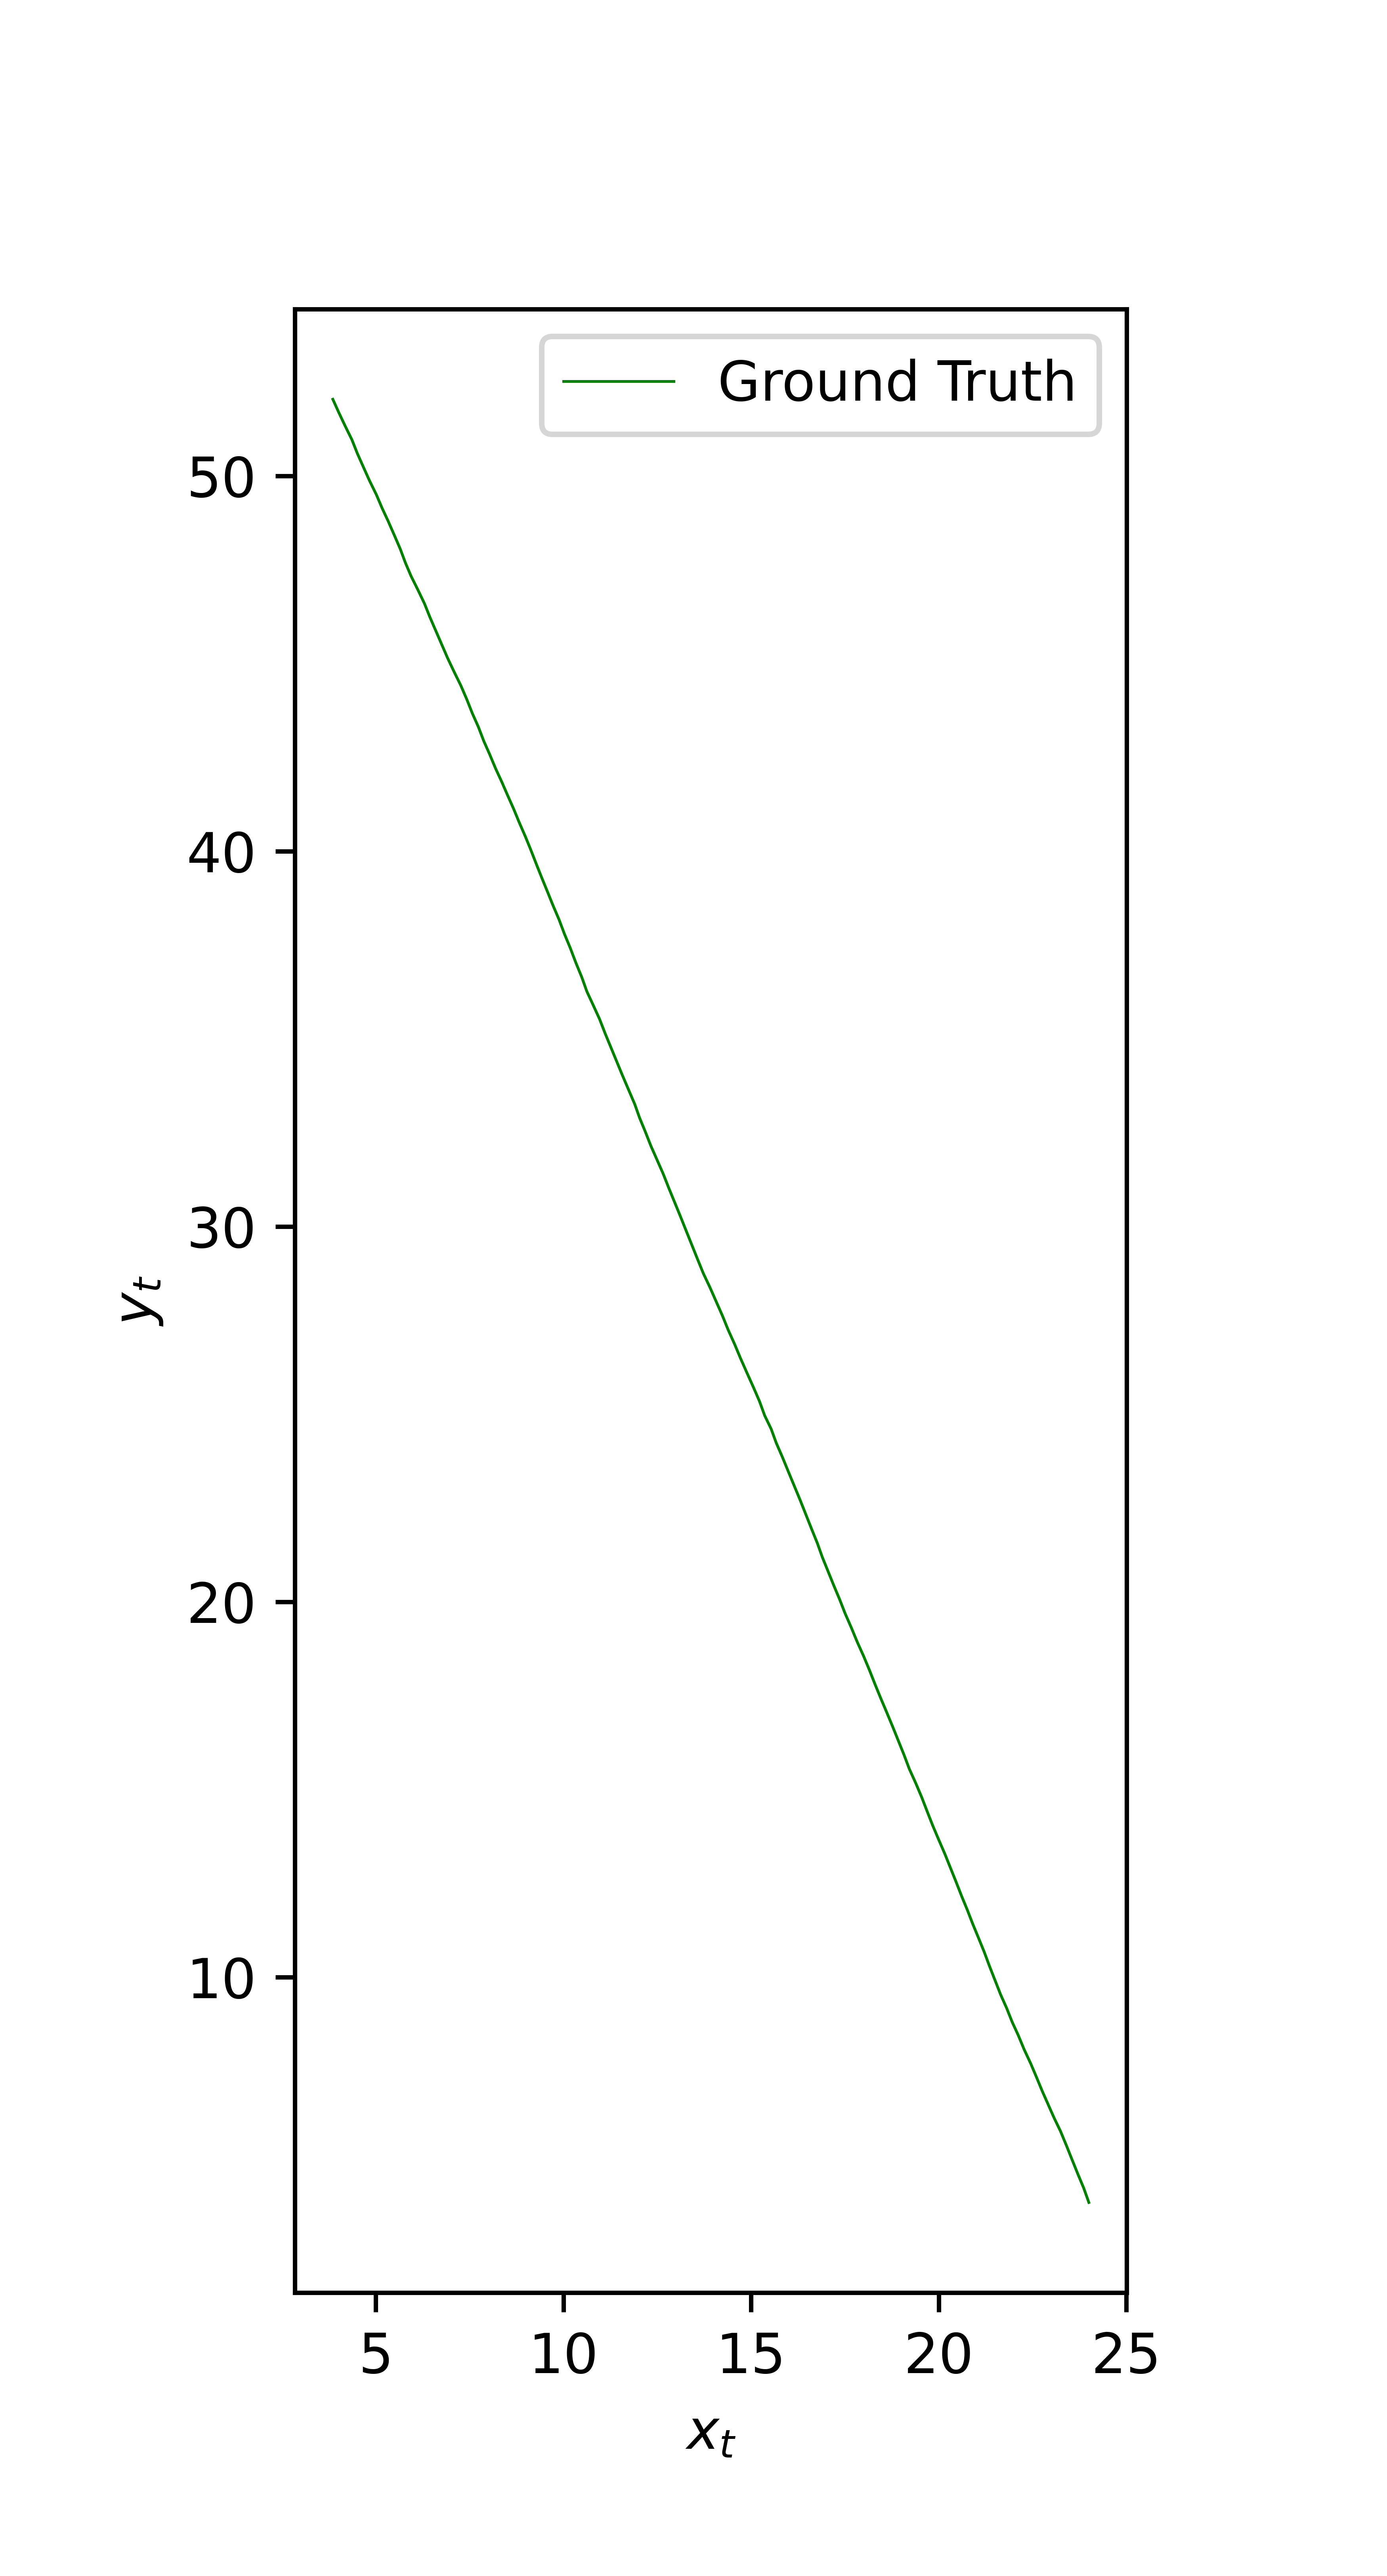
\includegraphics[width=1.2\linewidth]{plots/part2-e-GT.png}
        \caption*{Ground Truth trajectory}
    \end{minipage}
    \hfill
    \begin{minipage}{0.32\linewidth}
        \centering
        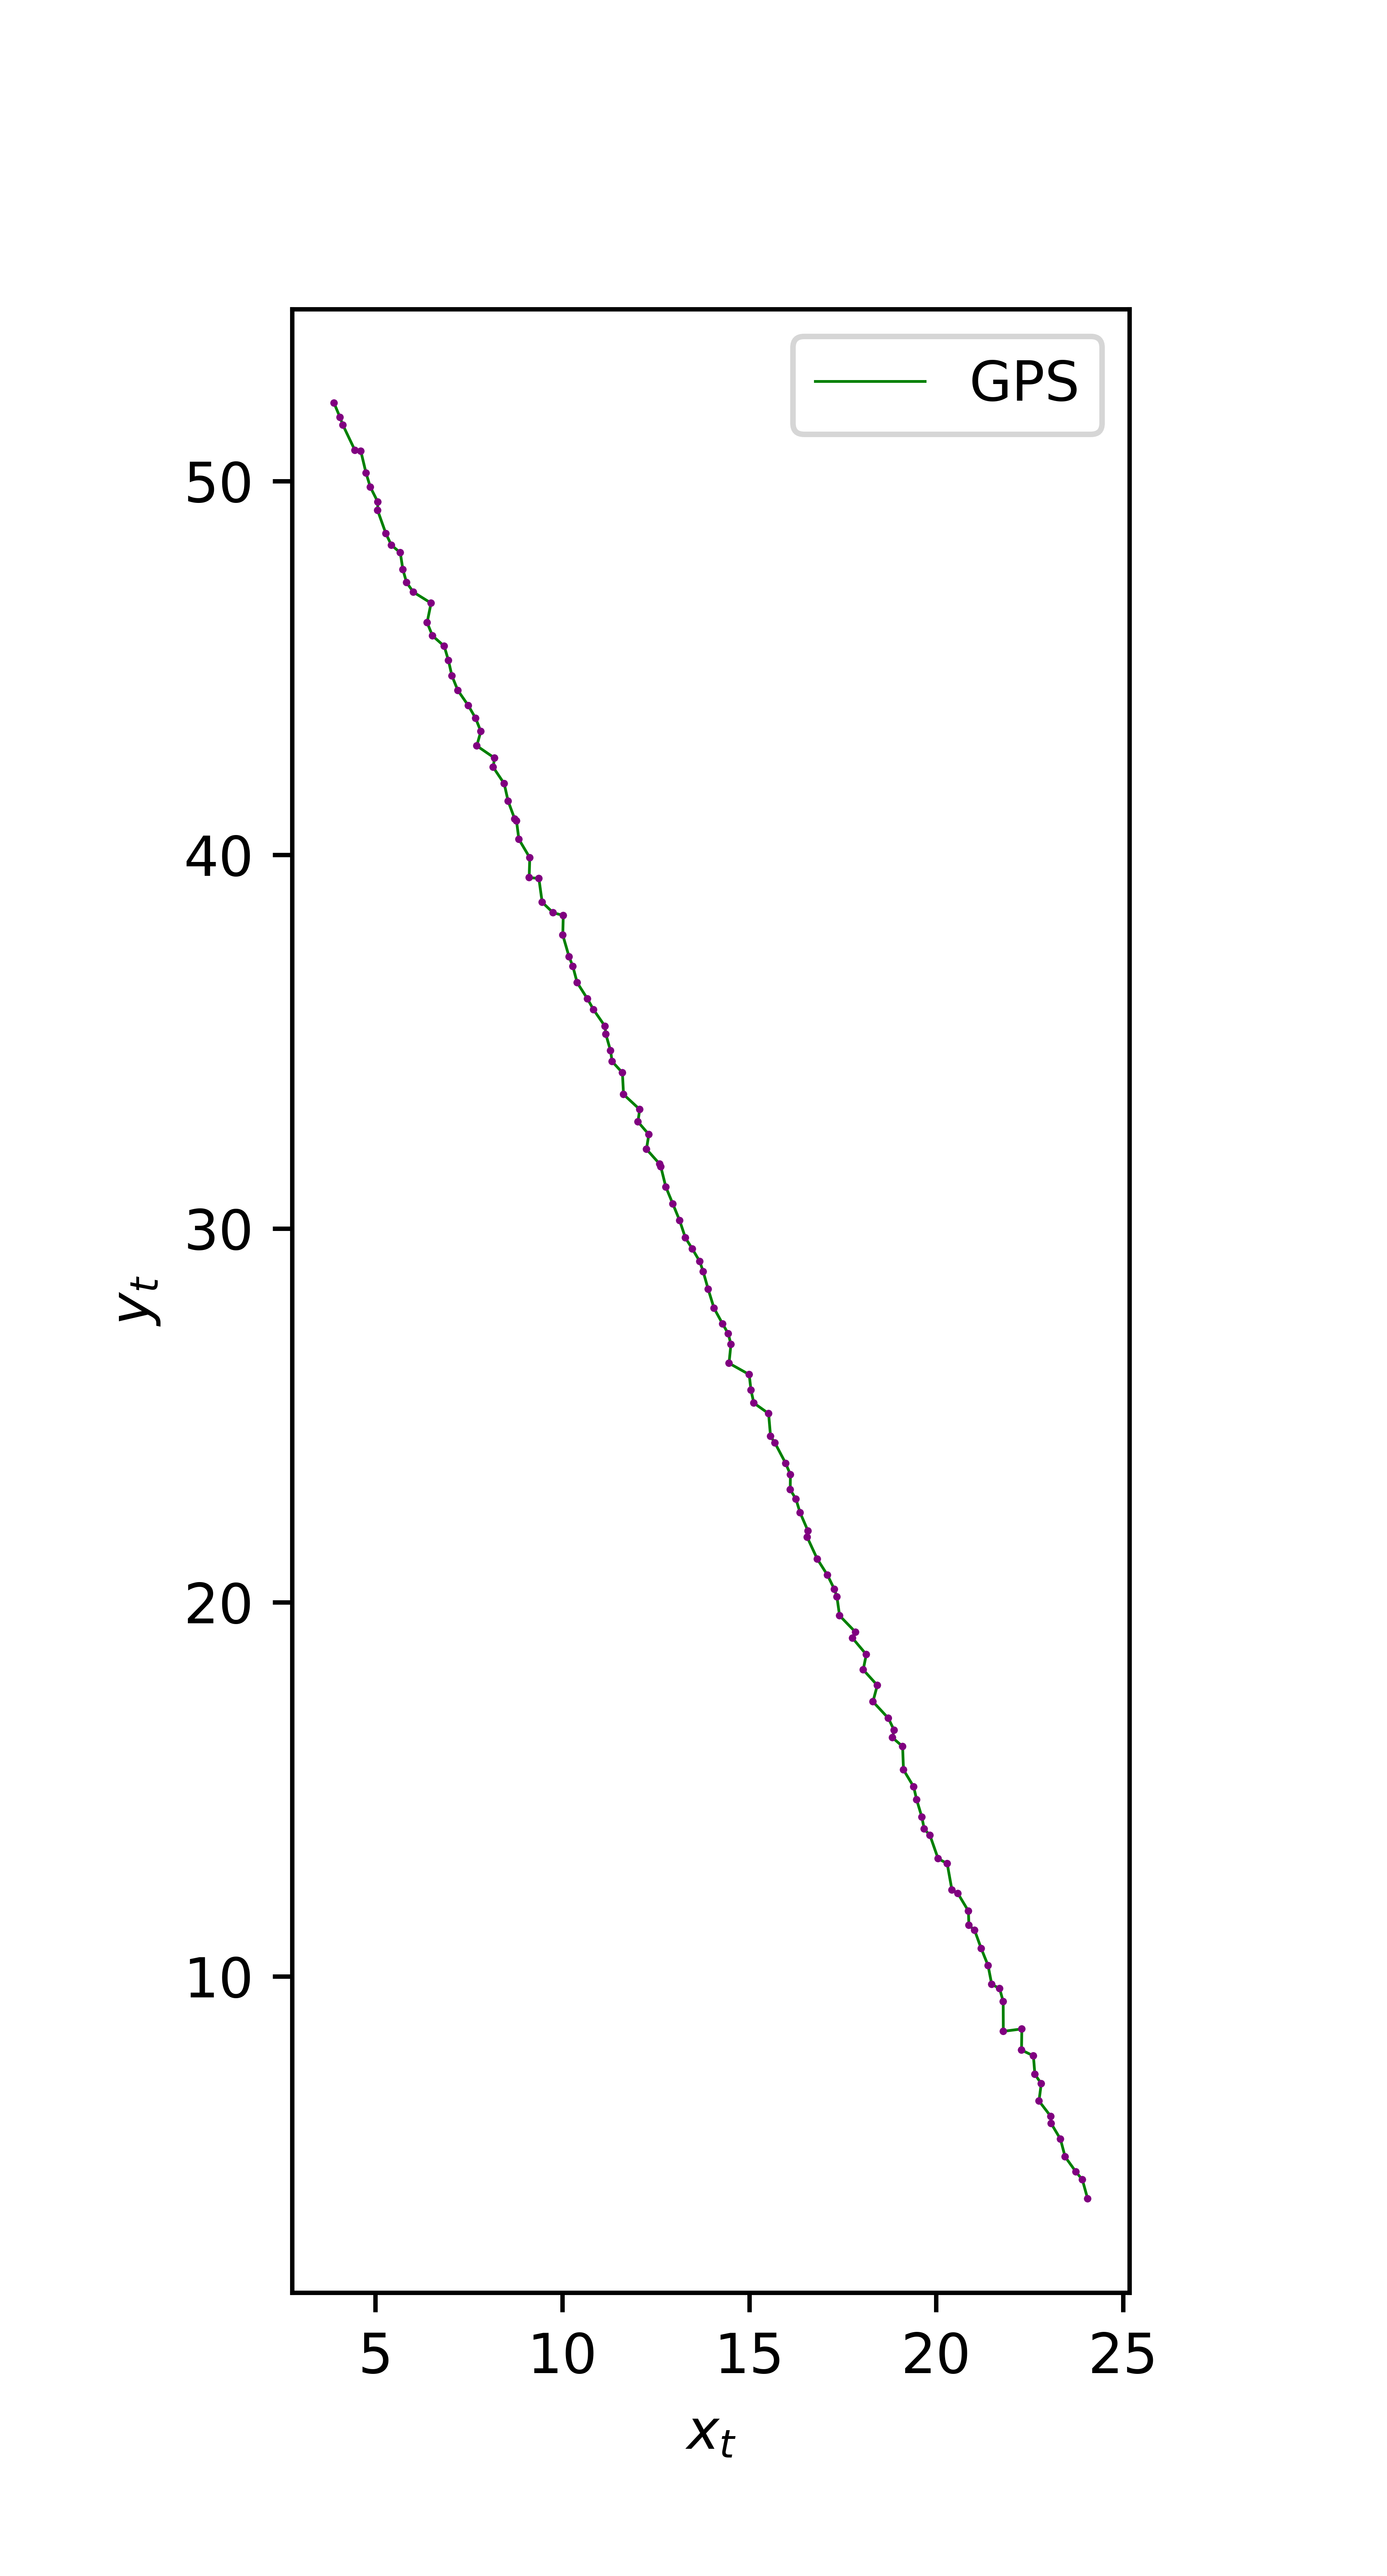
\includegraphics[width=1.2\linewidth]{plots/part2-e-GPS.png}
        \caption*{Trajectory using GPS observations}
    \end{minipage}
    \hfill
    \begin{minipage}{0.32\linewidth}
        \centering
        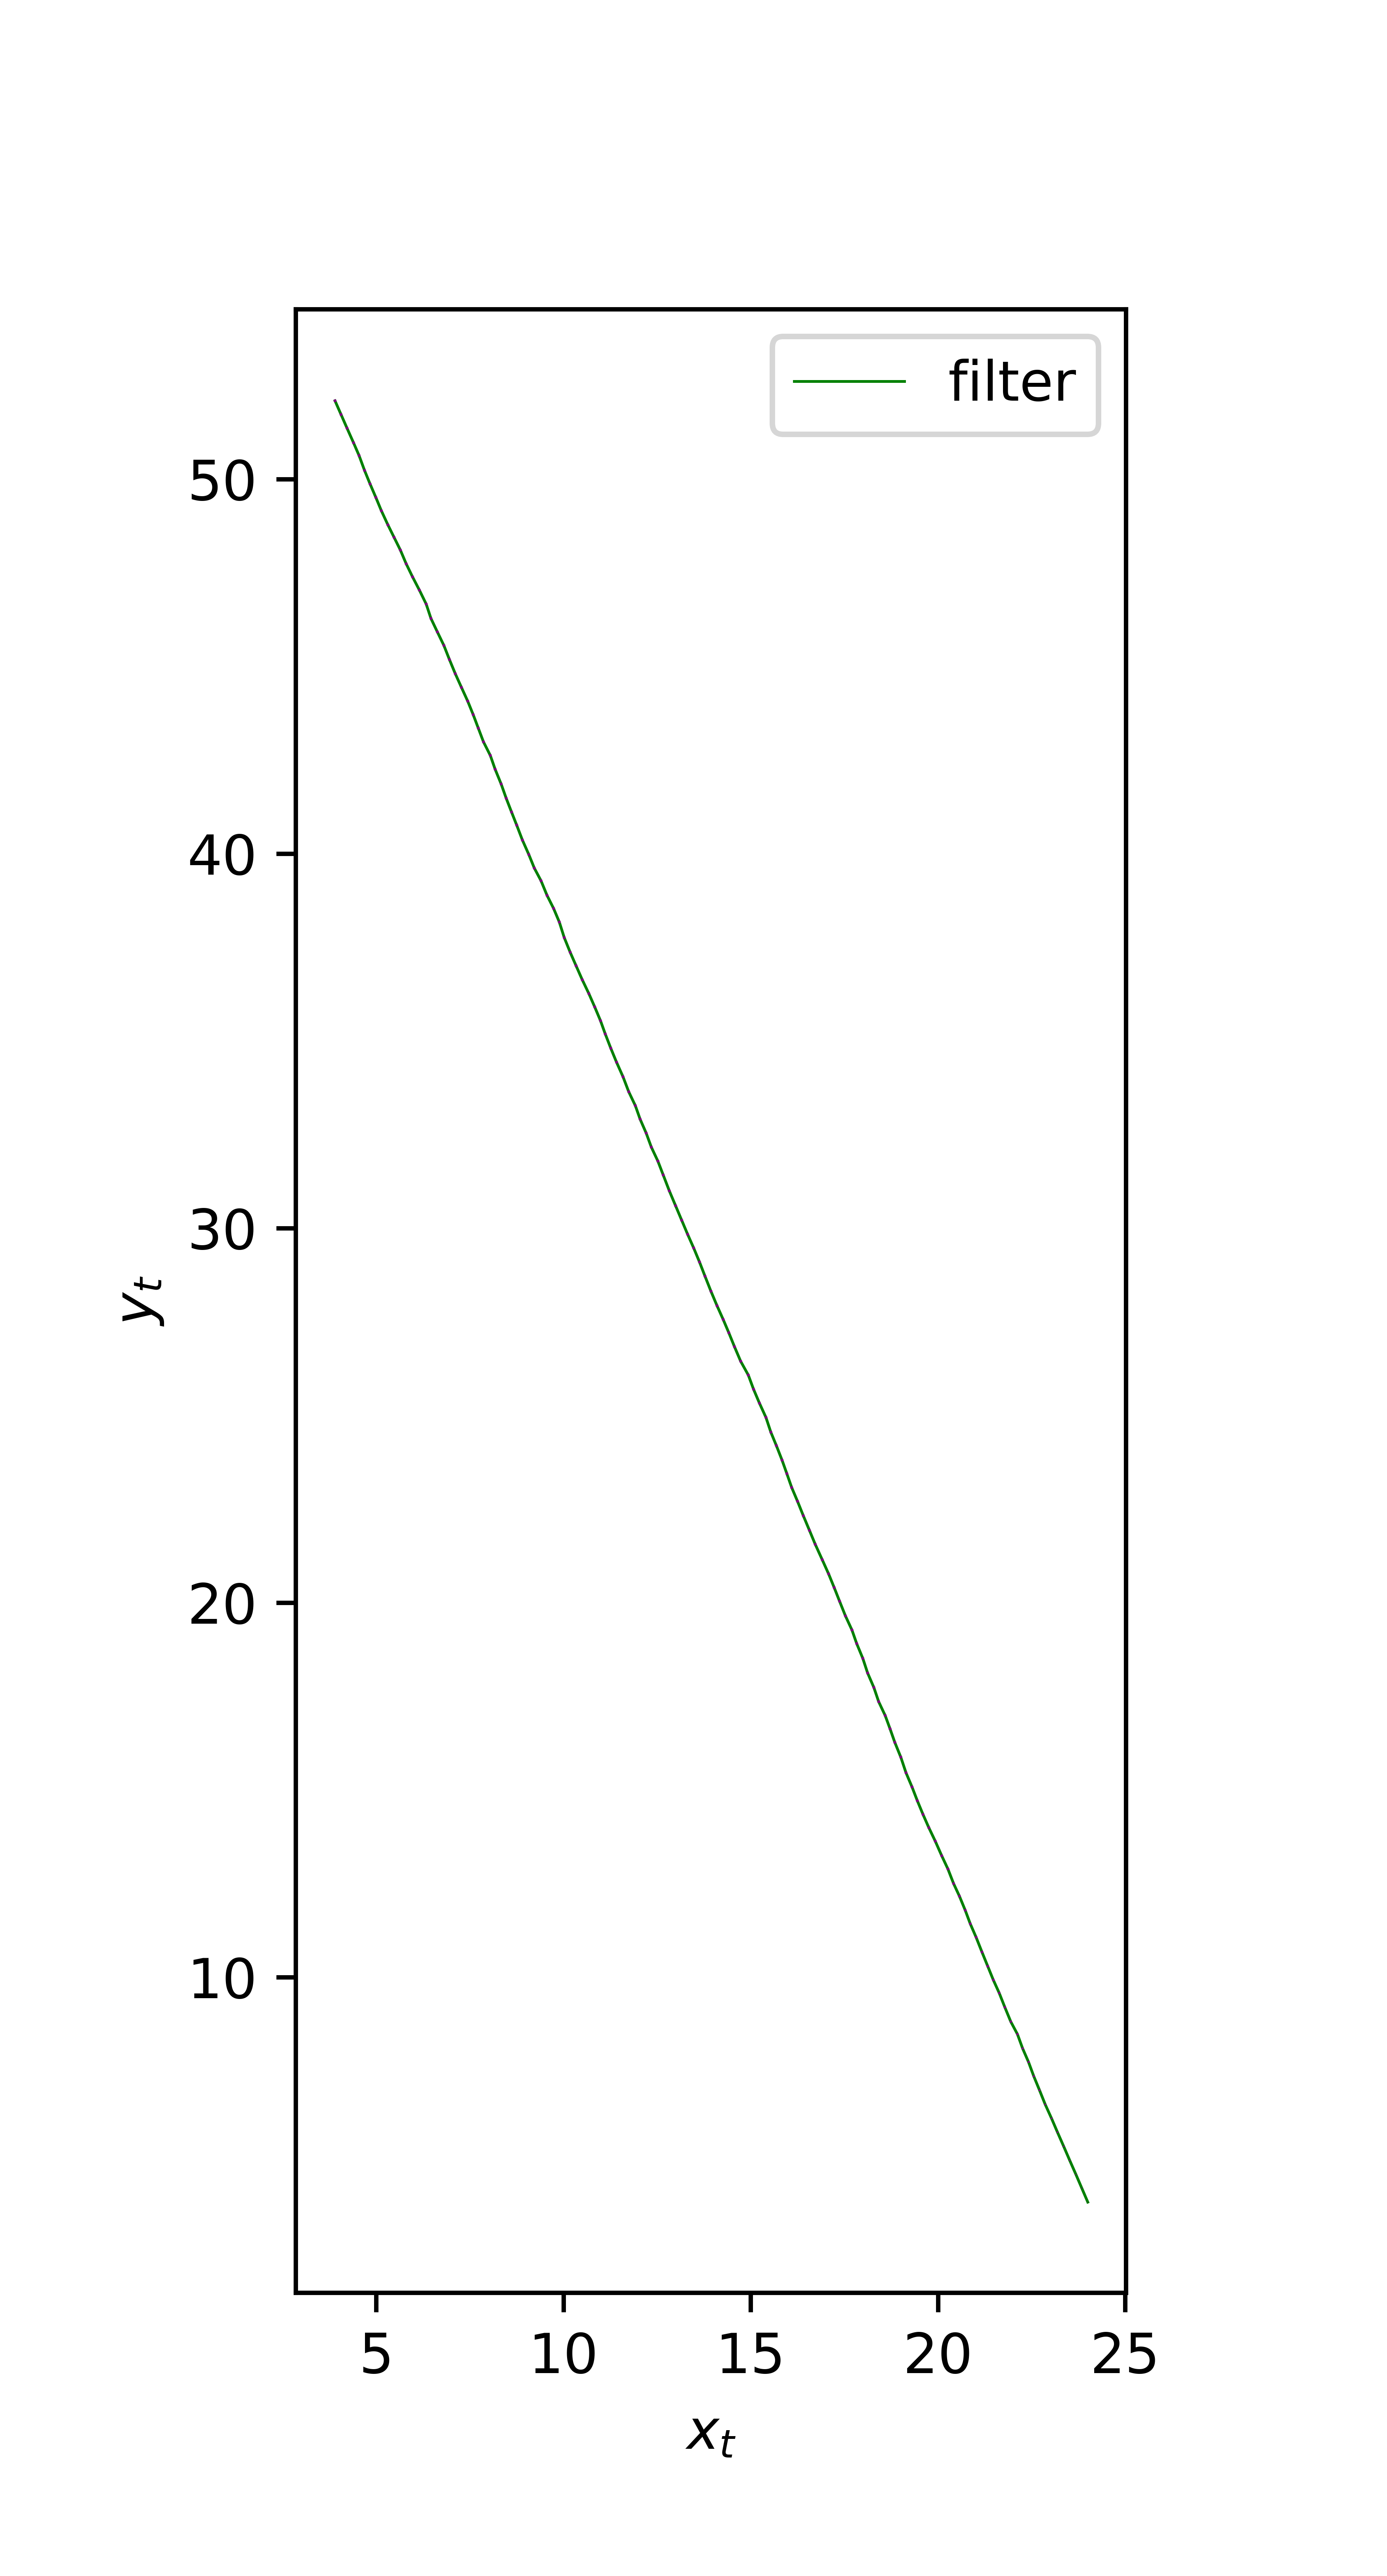
\includegraphics[width=1.2\linewidth]{plots/part2-e-filter.png}
        \caption*{Trajectory output by Kalman Filter}
    \end{minipage}
    \caption{Uncertainty ellipses}
    \label{fig:uncertainty-ellipses}
\end{figure}



\subsection{Base-Stations in 2D Kinematics}
\begin{enumerate}
    \item In case of single BS sensors, for any point on the trajectory, the minor axis of the corresponding uncertainty ellipse is nearly in direction of that line joining the BS sensor to that point on the trajectory.

    \item Let the BS be at origin and the vector from BS sensor to point on trajectory be $\vec{d}$. For the same small step size $\alpha$, movement also $\vec{d}$ changes sensor observation by larger amount ($= \alpha$) compared to moving perpendicular to $\vec{d}$ ($= \sqrt{d^2 + \alpha^2} - d$). Hence, given sensor observation, if actual value deviates along $\vec{d}$, it is likely deviates less, as the distance increases rapidy in this direction, while the range $[x^e - \sigma_{x^e}, x^e + \sigma_{x^e}]$ is fixed.
    
\item The minor axis falls sharply in all cases. The major axis seems to have a minimum when the point is closest to the sensor.
\end{enumerate}
\begin{figure}[H]
    \centering
    \begin{minipage}{0.49\linewidth}
        \centering
        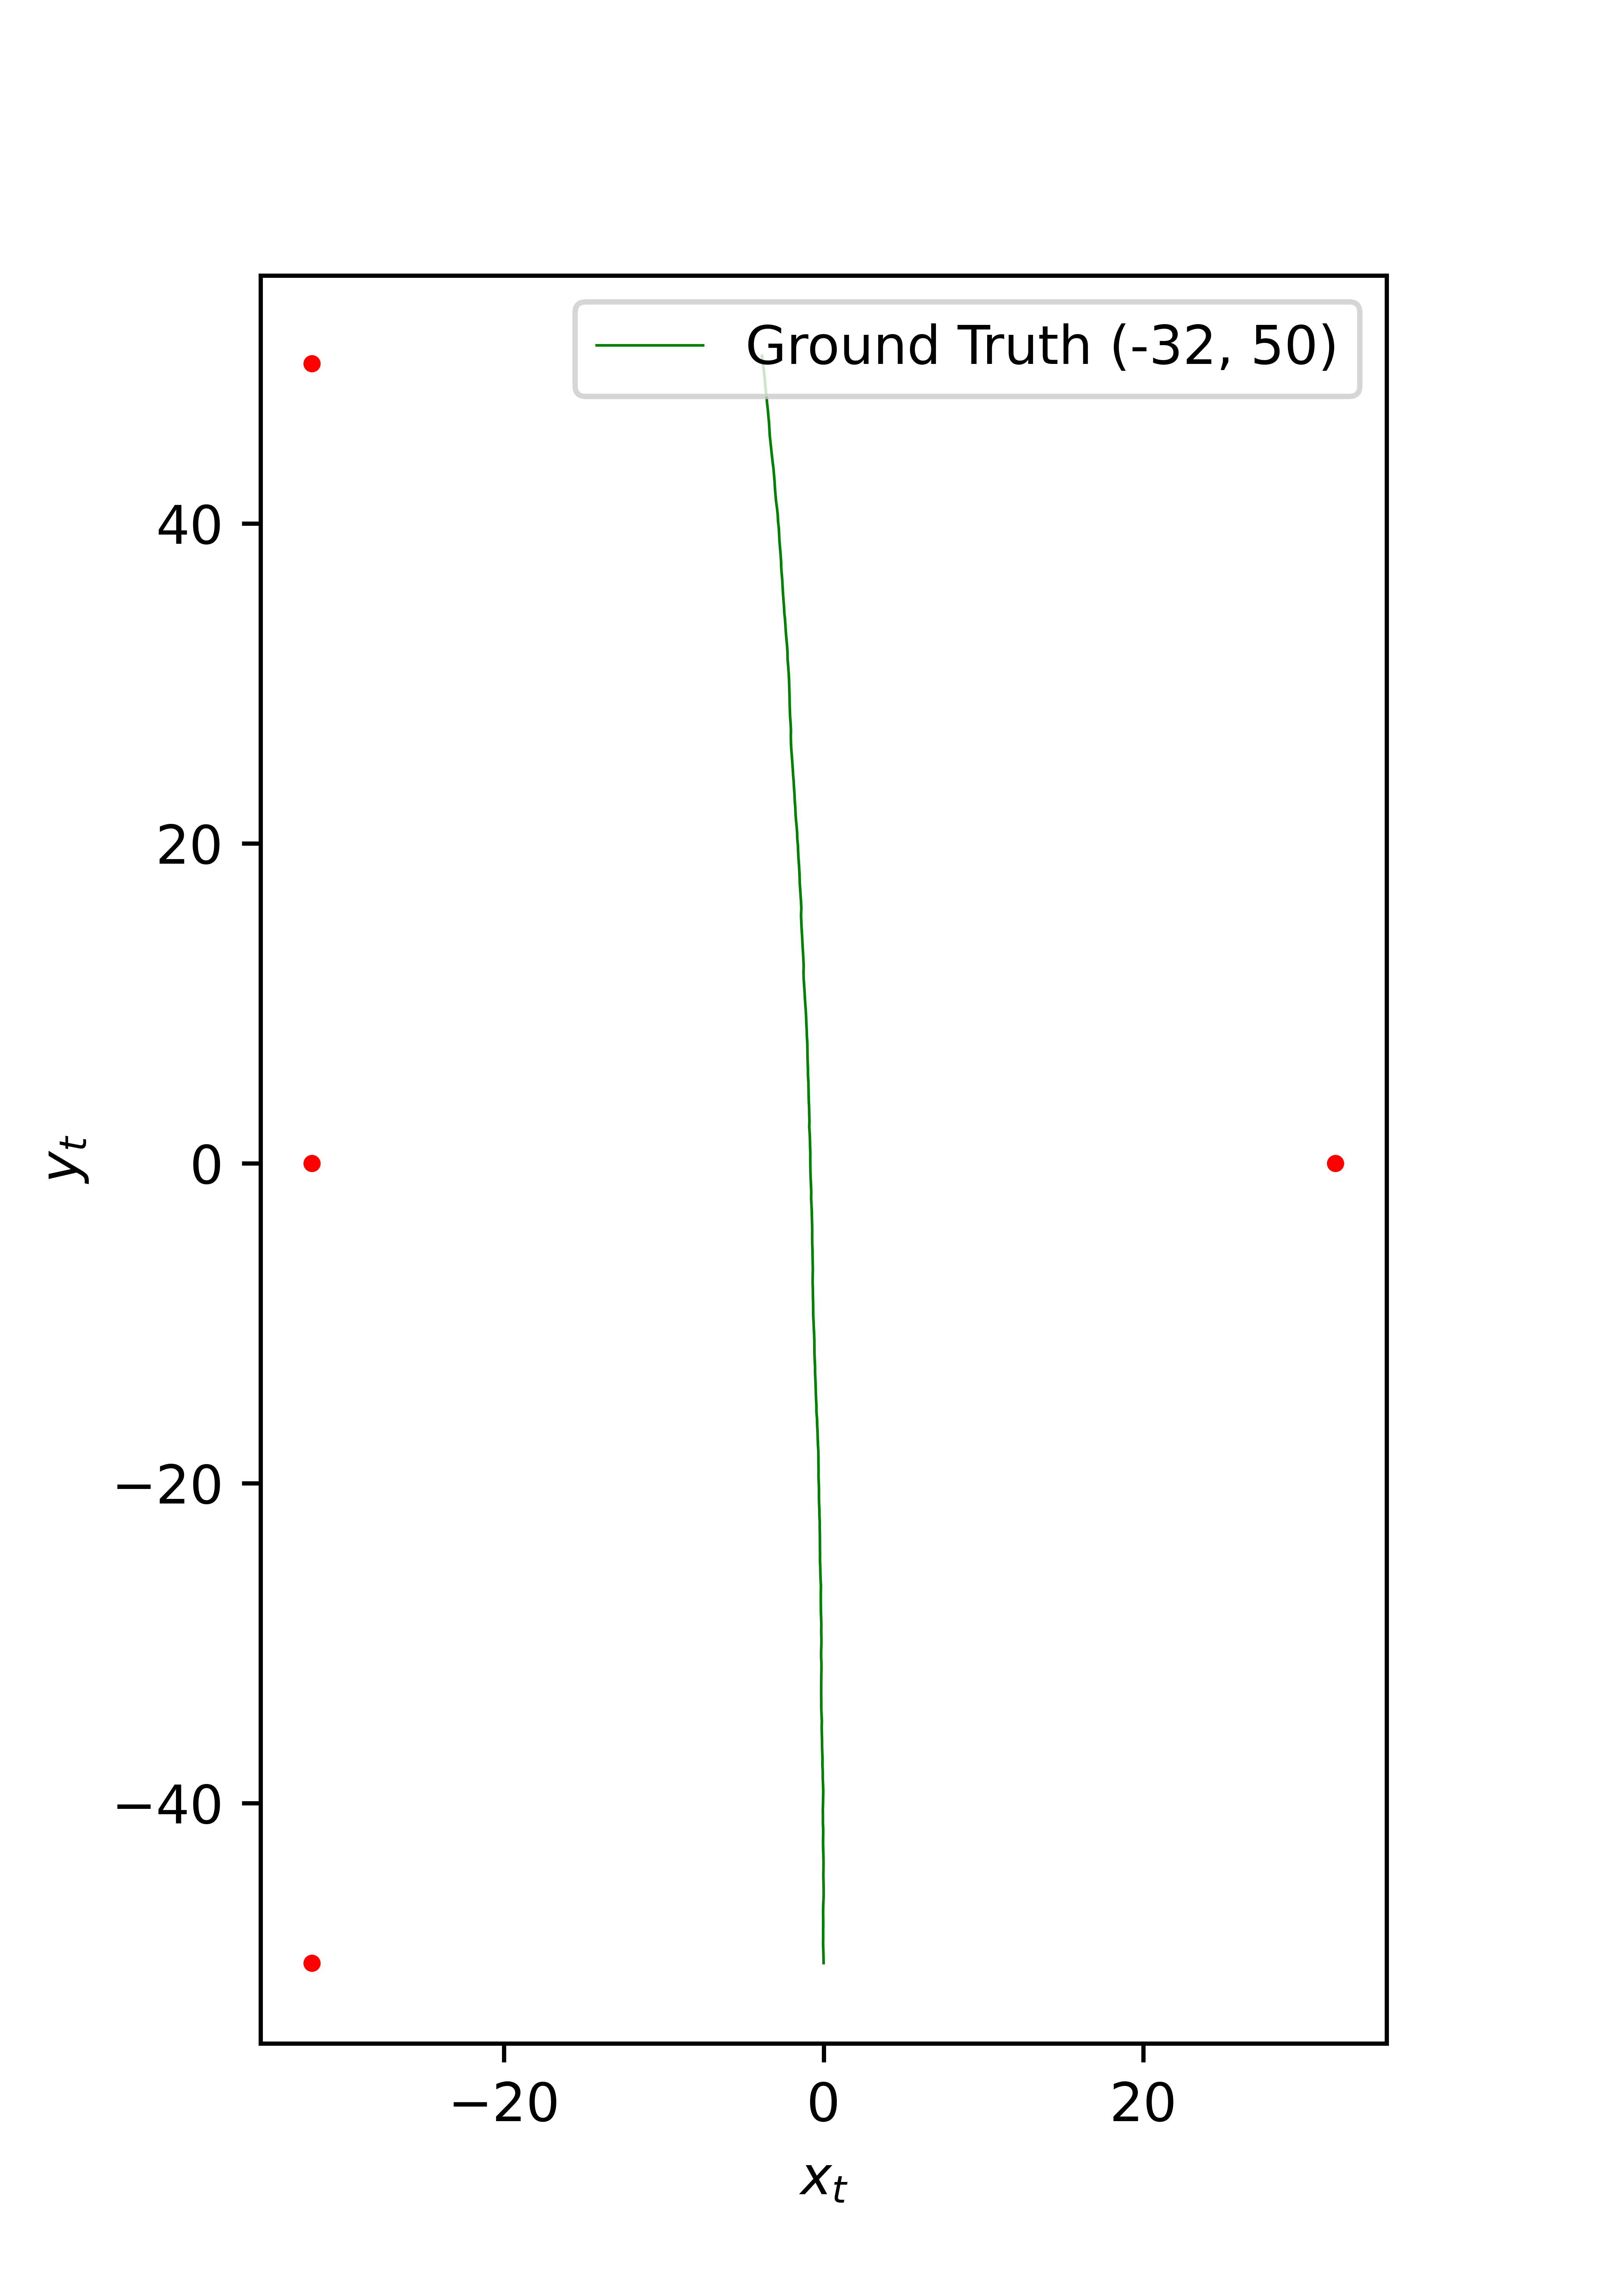
\includegraphics[width=\linewidth]{plots/part2-f-0-GT.png}
        \caption*{Ground Truth}
    \end{minipage}
    \hfill
    \begin{minipage}{0.49\linewidth}
        \centering
        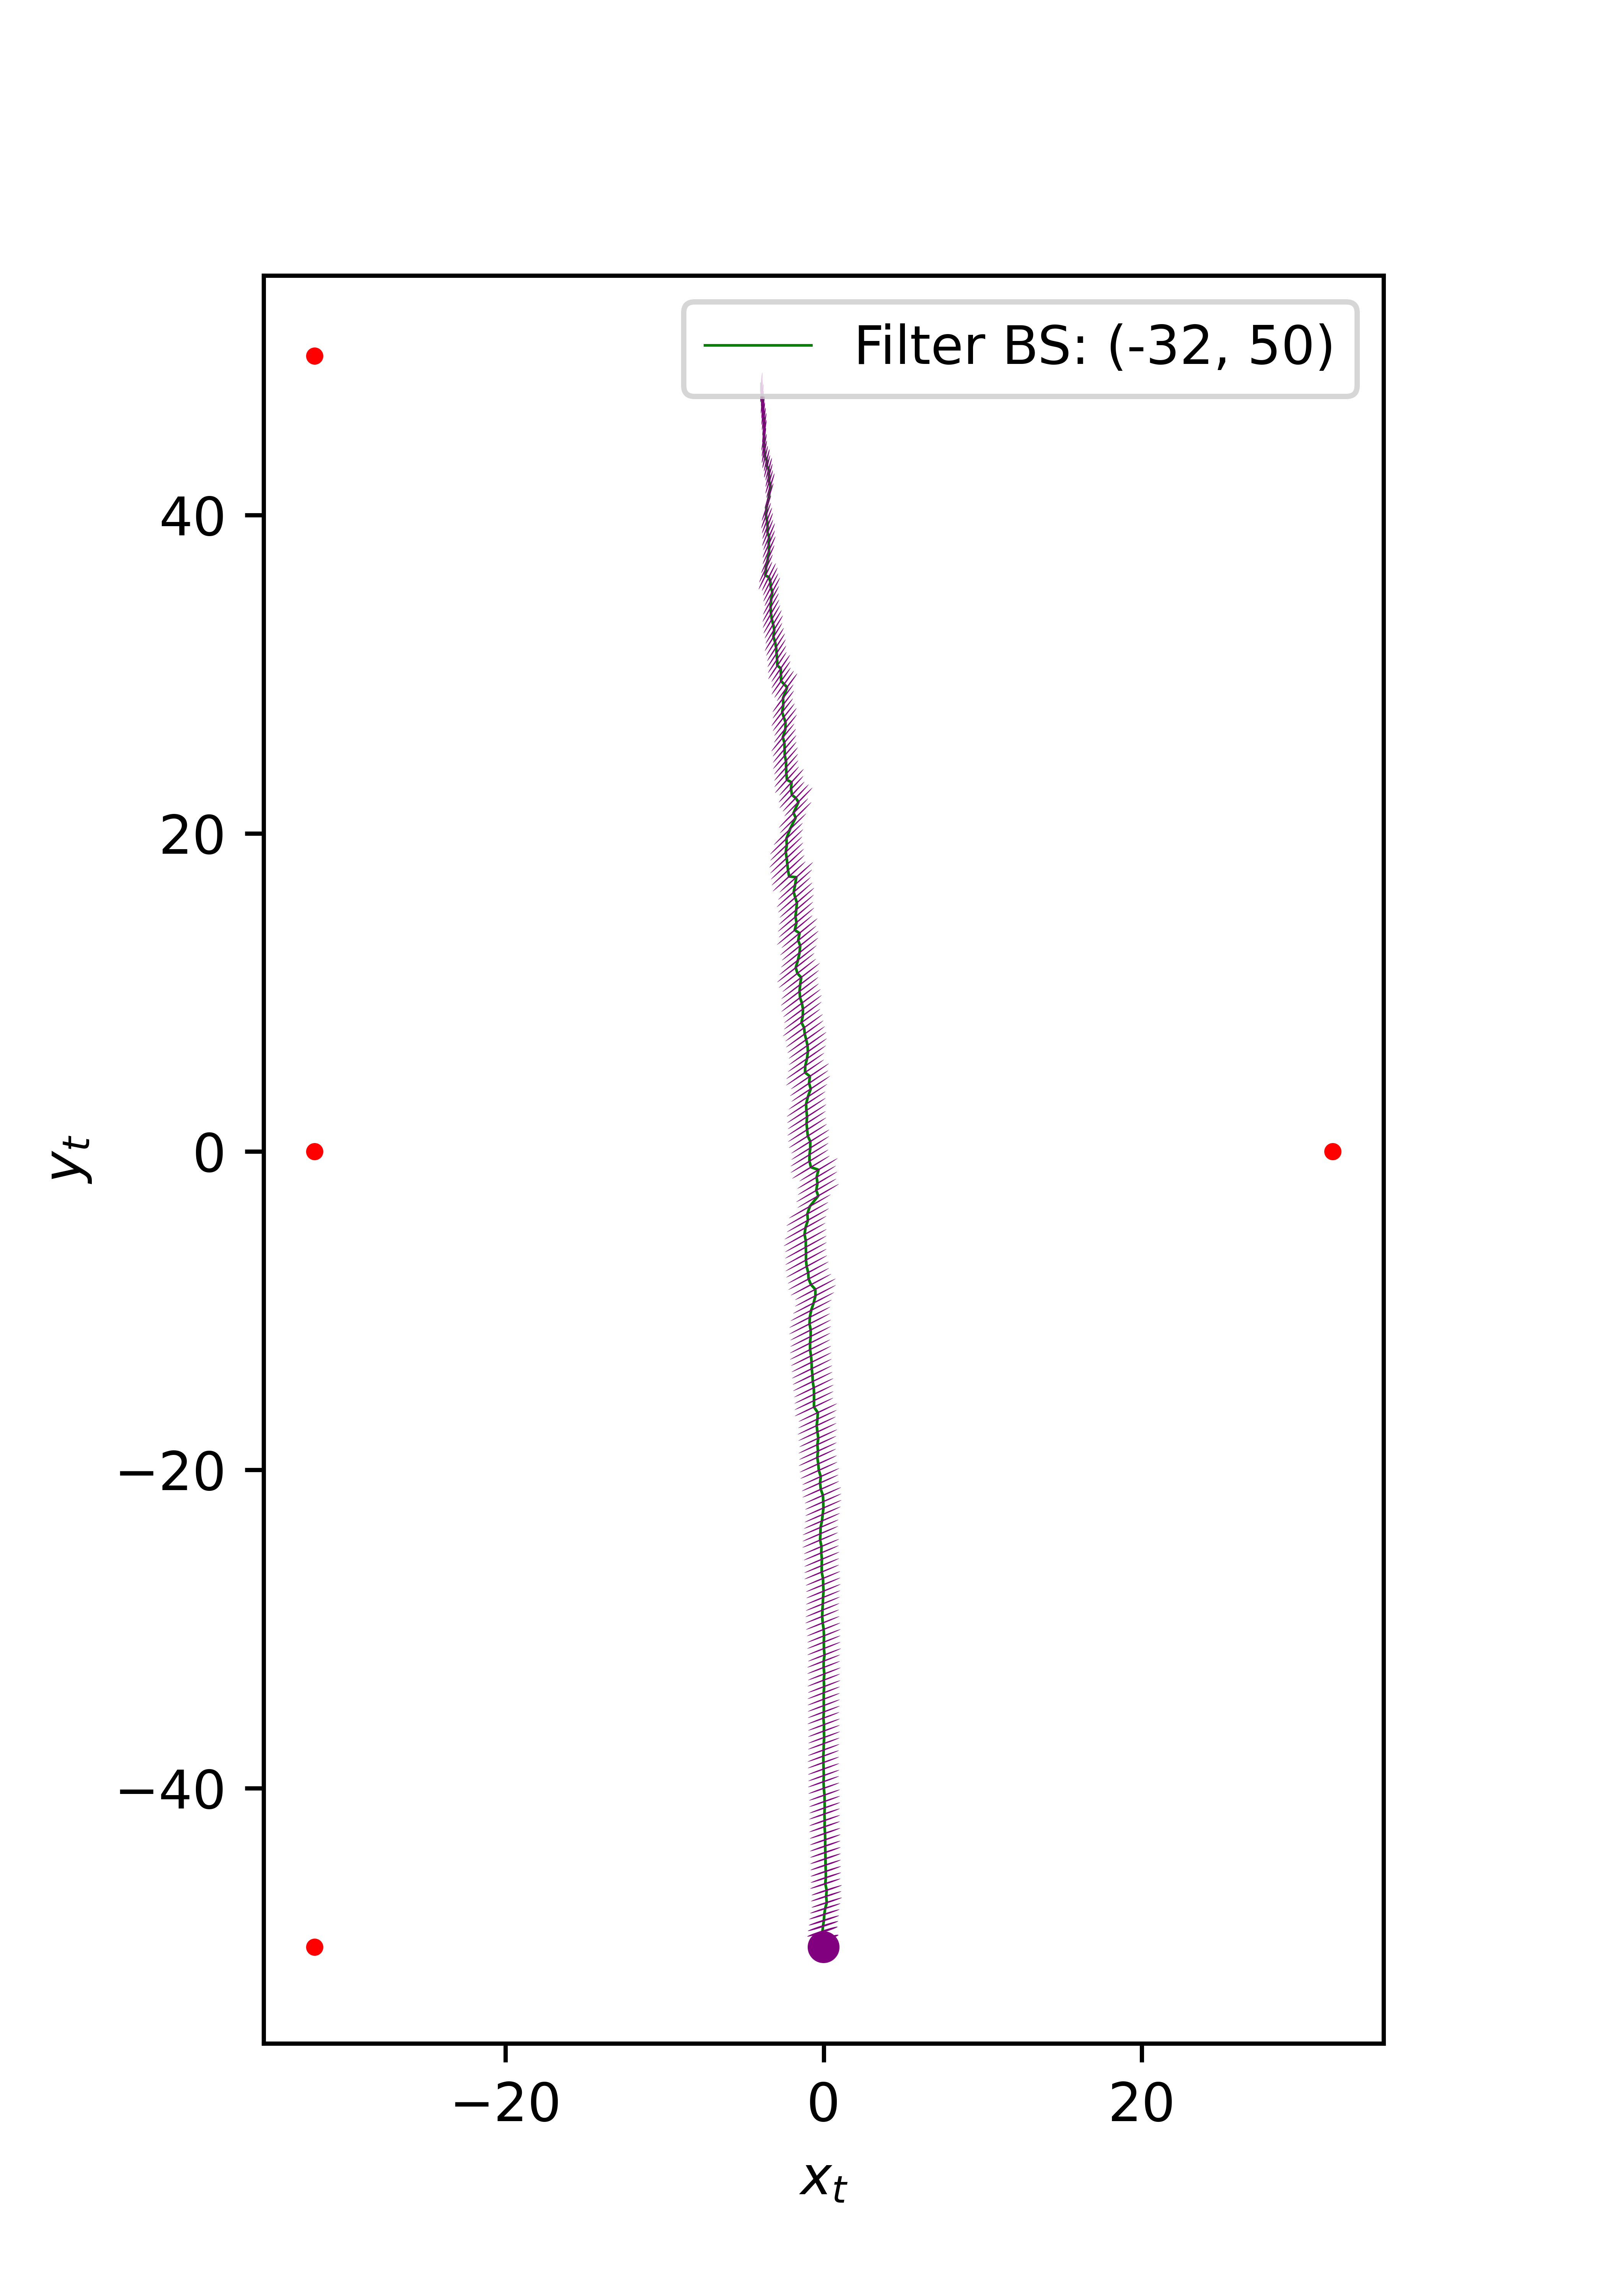
\includegraphics[width=\linewidth]{plots/part2-f-0-filter.png}
        \caption*{Kalman Filter}
    \end{minipage}

    \vspace{-0.1cm}
    \begin{minipage}{\linewidth}
        \centering
        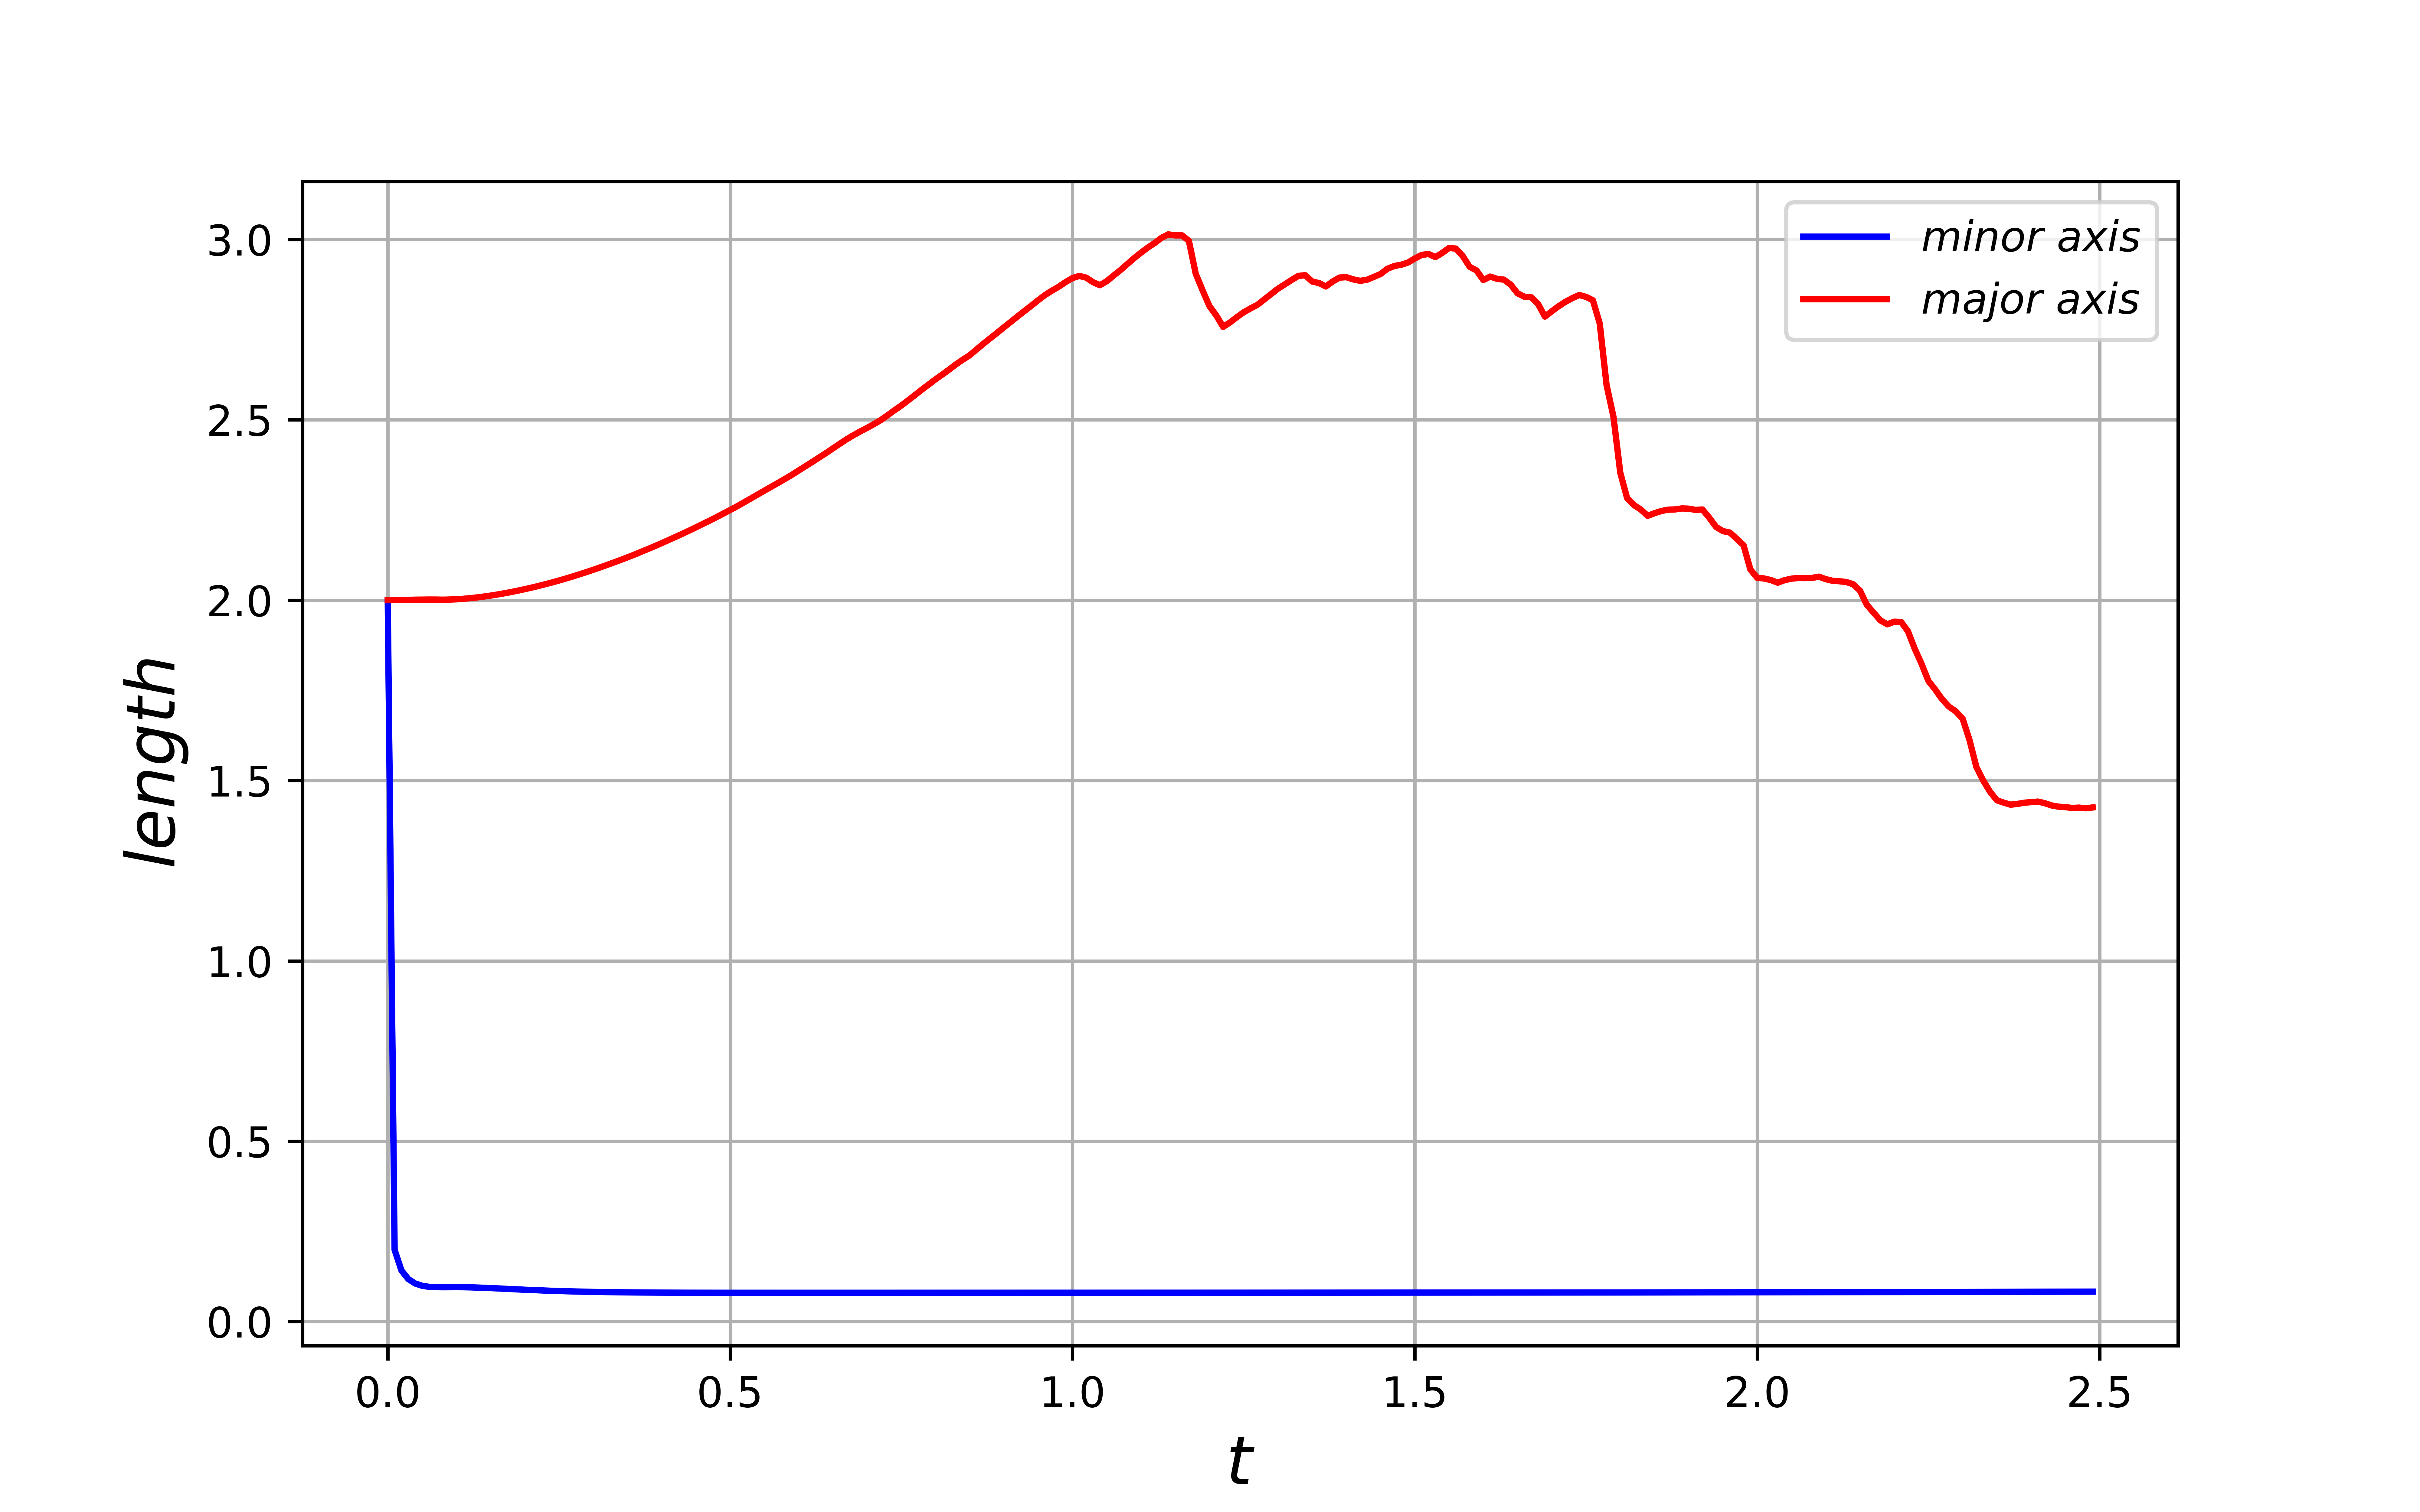
\includegraphics[width=\linewidth]{plots/part2-f-0-axes.png}
        \caption*{Major and Minor Axes}
    \end{minipage}

    \caption{Base-Station $B_1(-32, 50)$}
\end{figure}



\begin{figure}[H]
    \centering
    \begin{minipage}{0.49\linewidth}
        \centering
        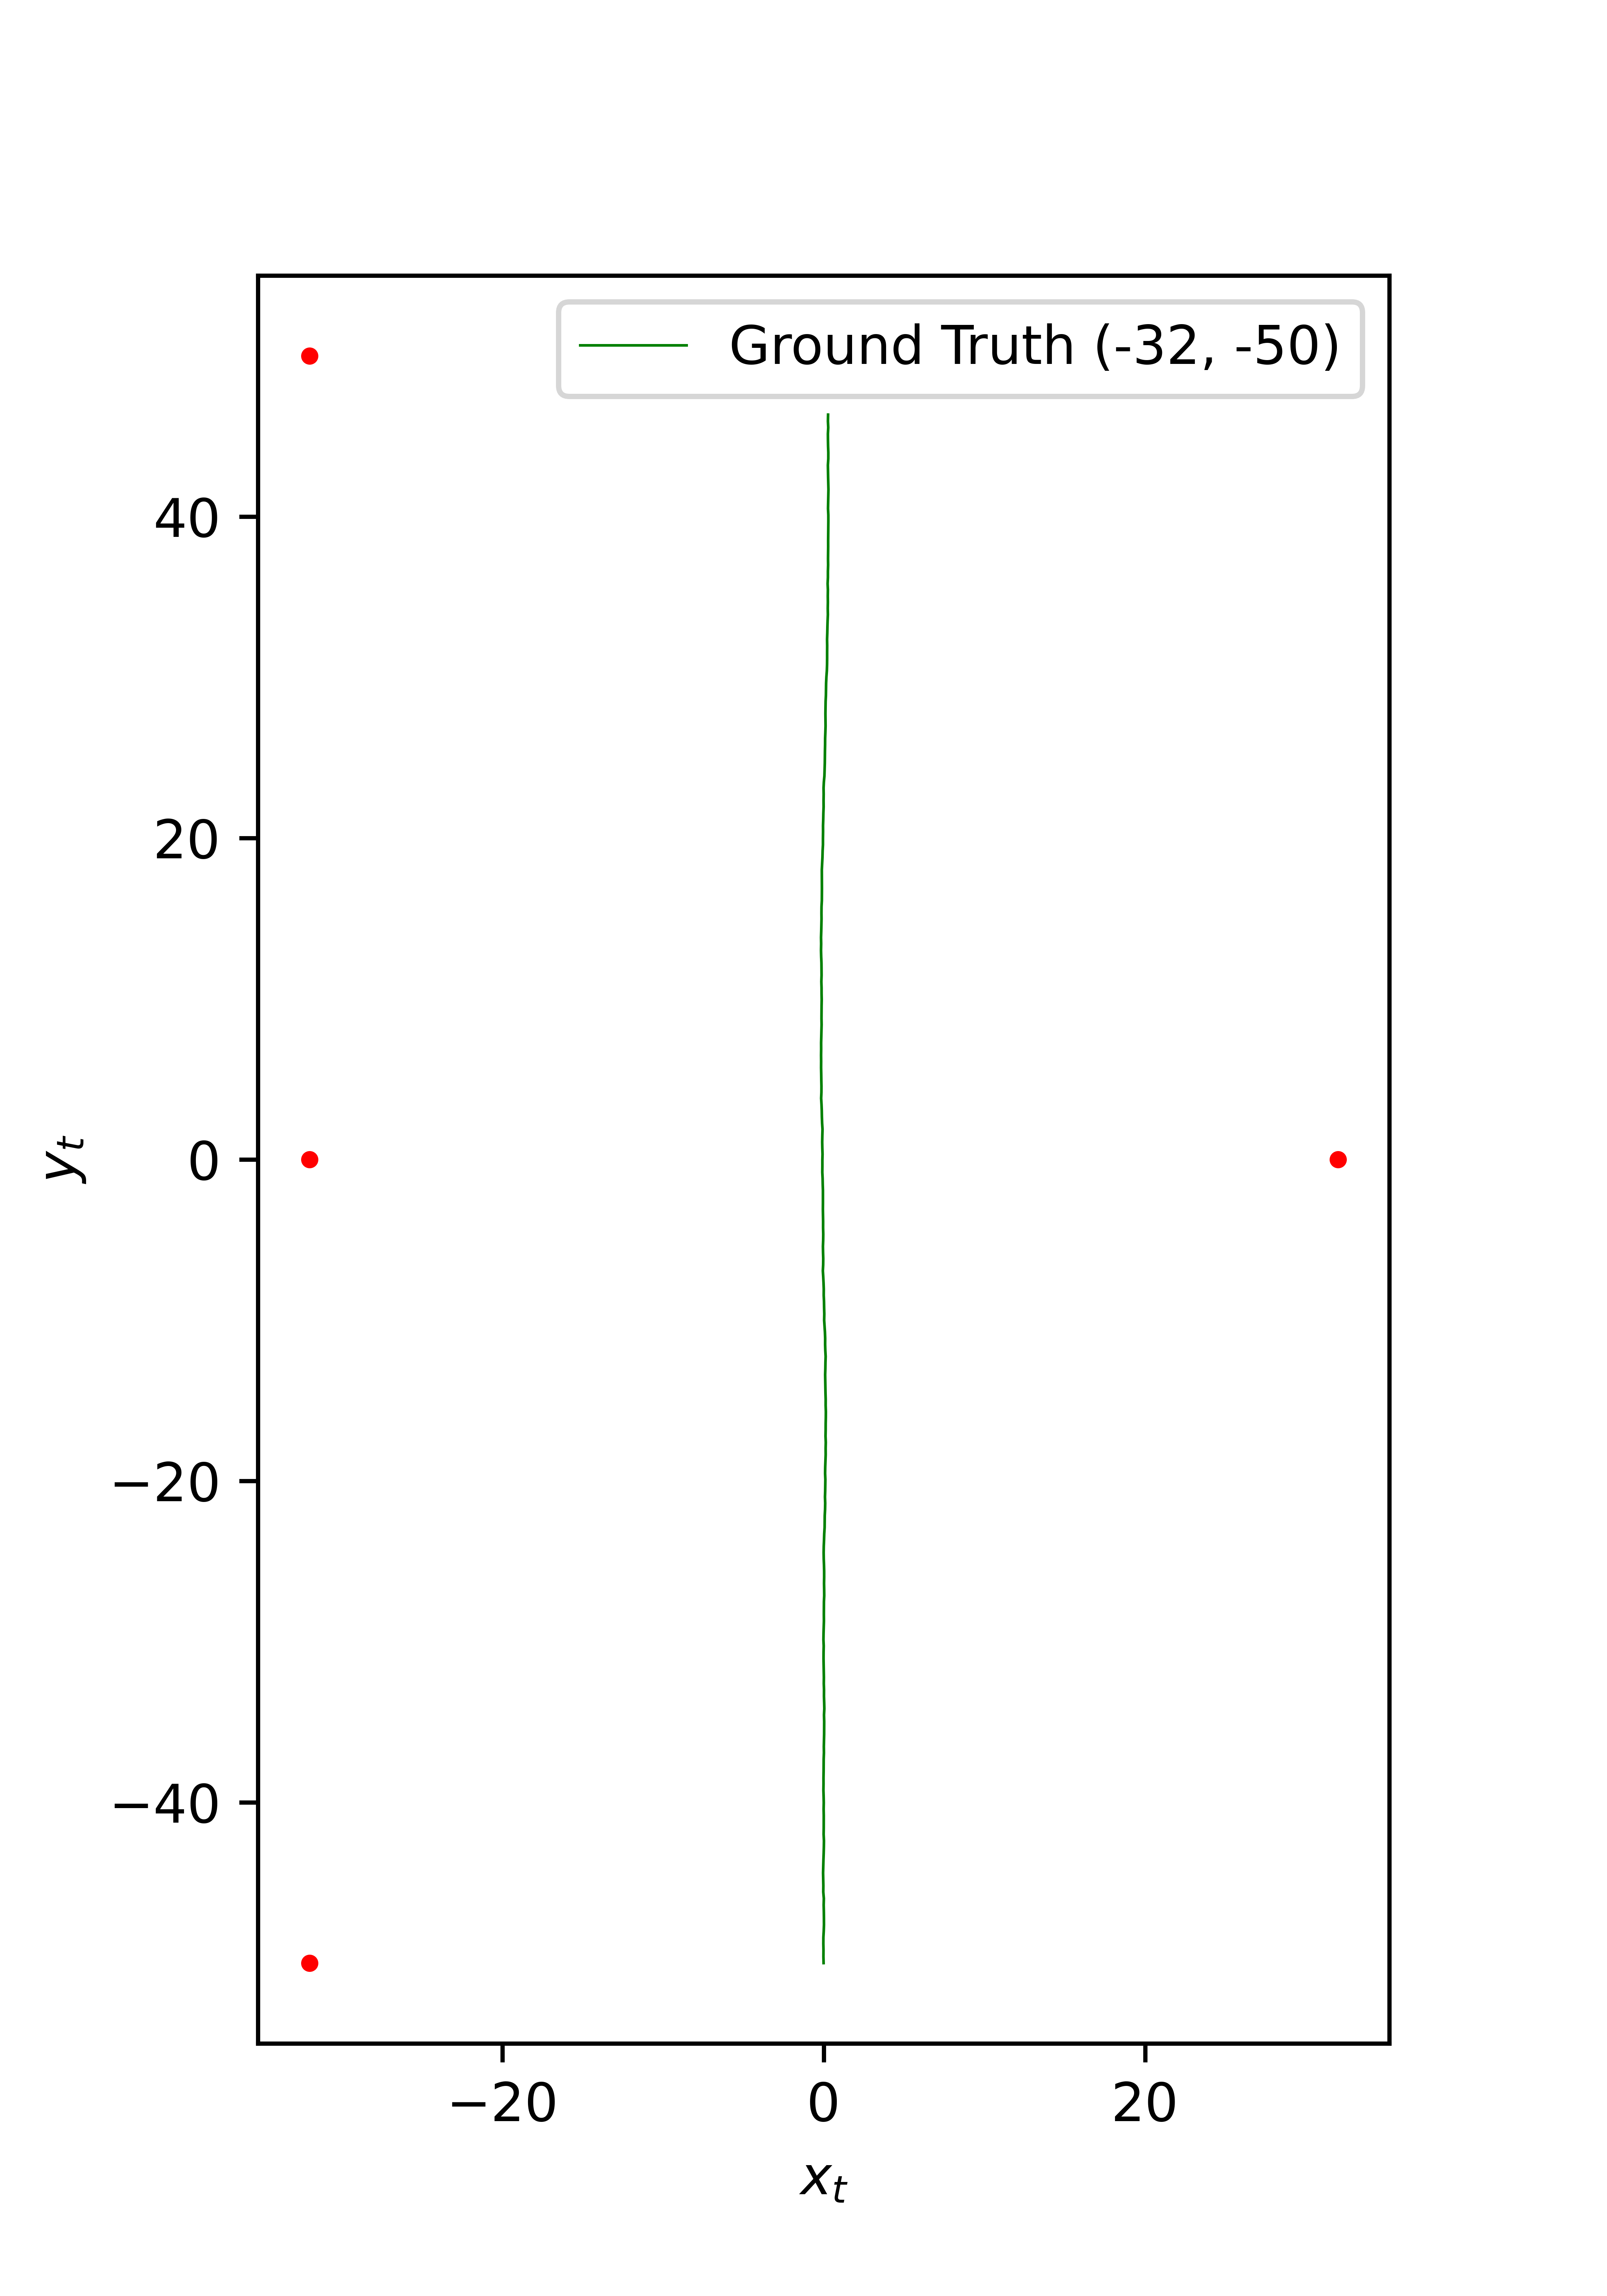
\includegraphics[width=\linewidth]{plots/part2-f-1-GT.png}
        \caption*{Ground Truth}
    \end{minipage}
    \hfill
    \begin{minipage}{0.49\linewidth}
        \centering
        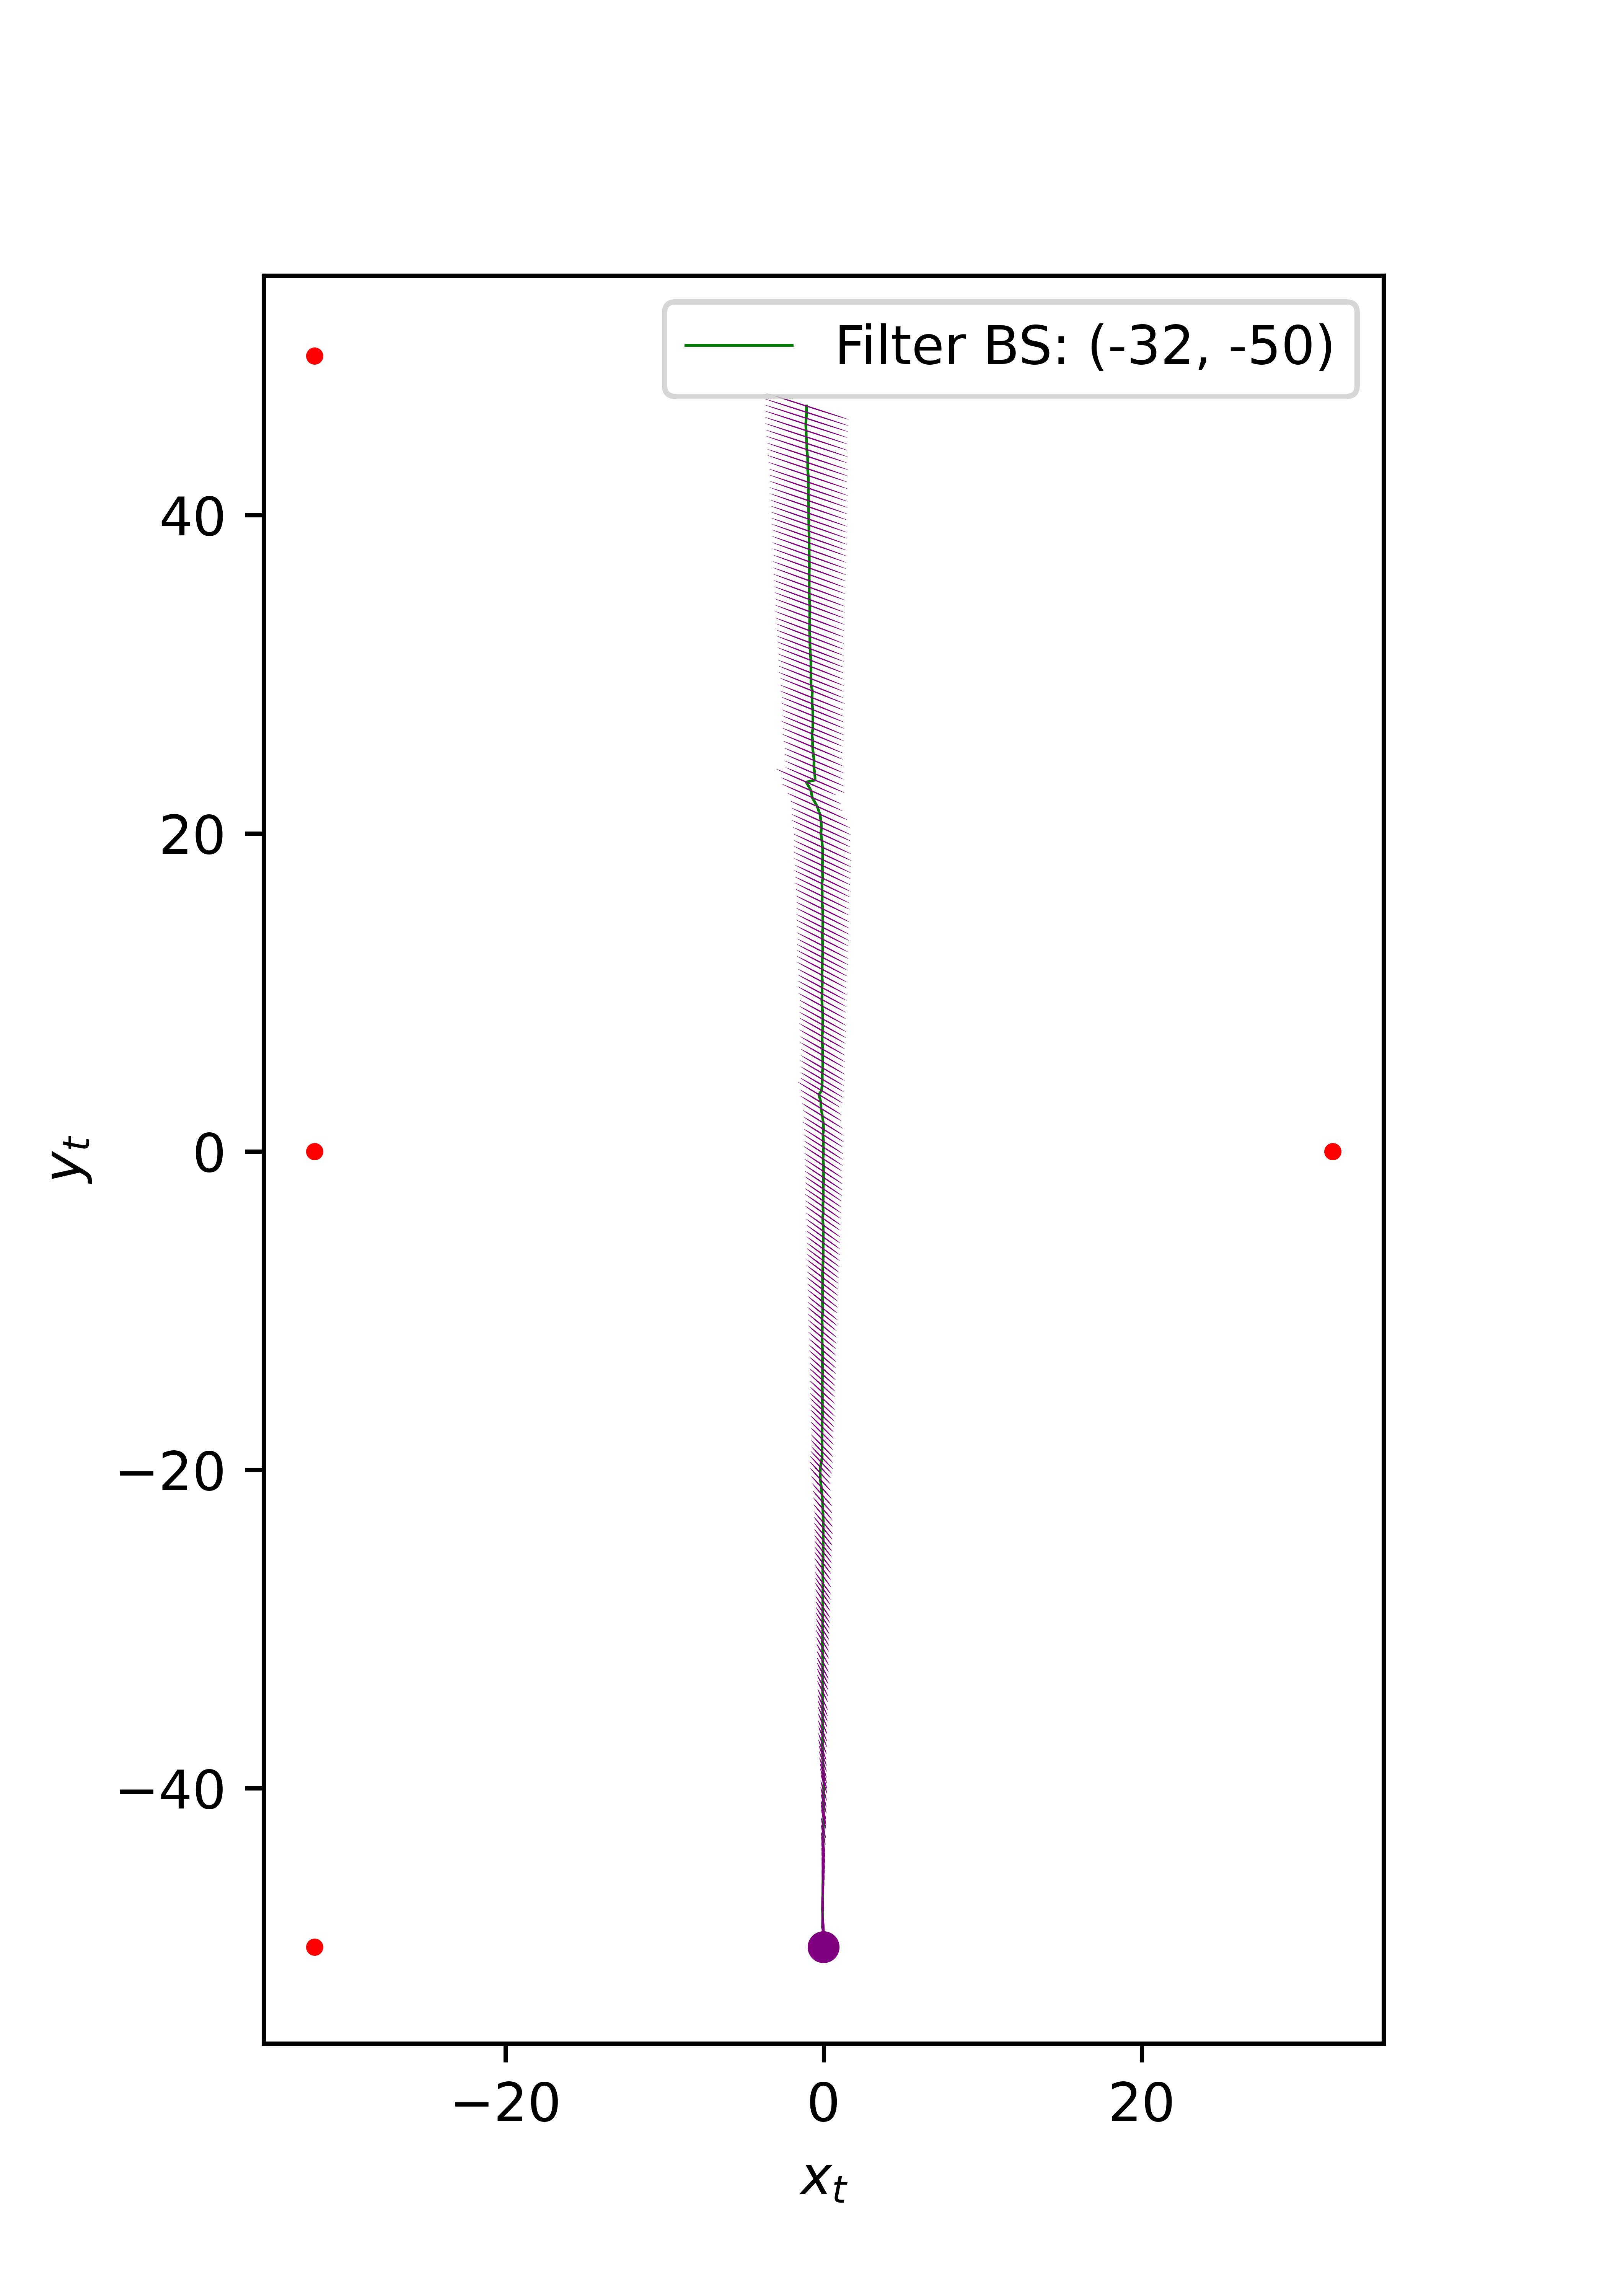
\includegraphics[width=\linewidth]{plots/part2-f-1-filter.png}
        \caption*{Kalman Filter}
    \end{minipage}
    \vspace{-0.1cm}
    \begin{minipage}{\linewidth}
        \centering
        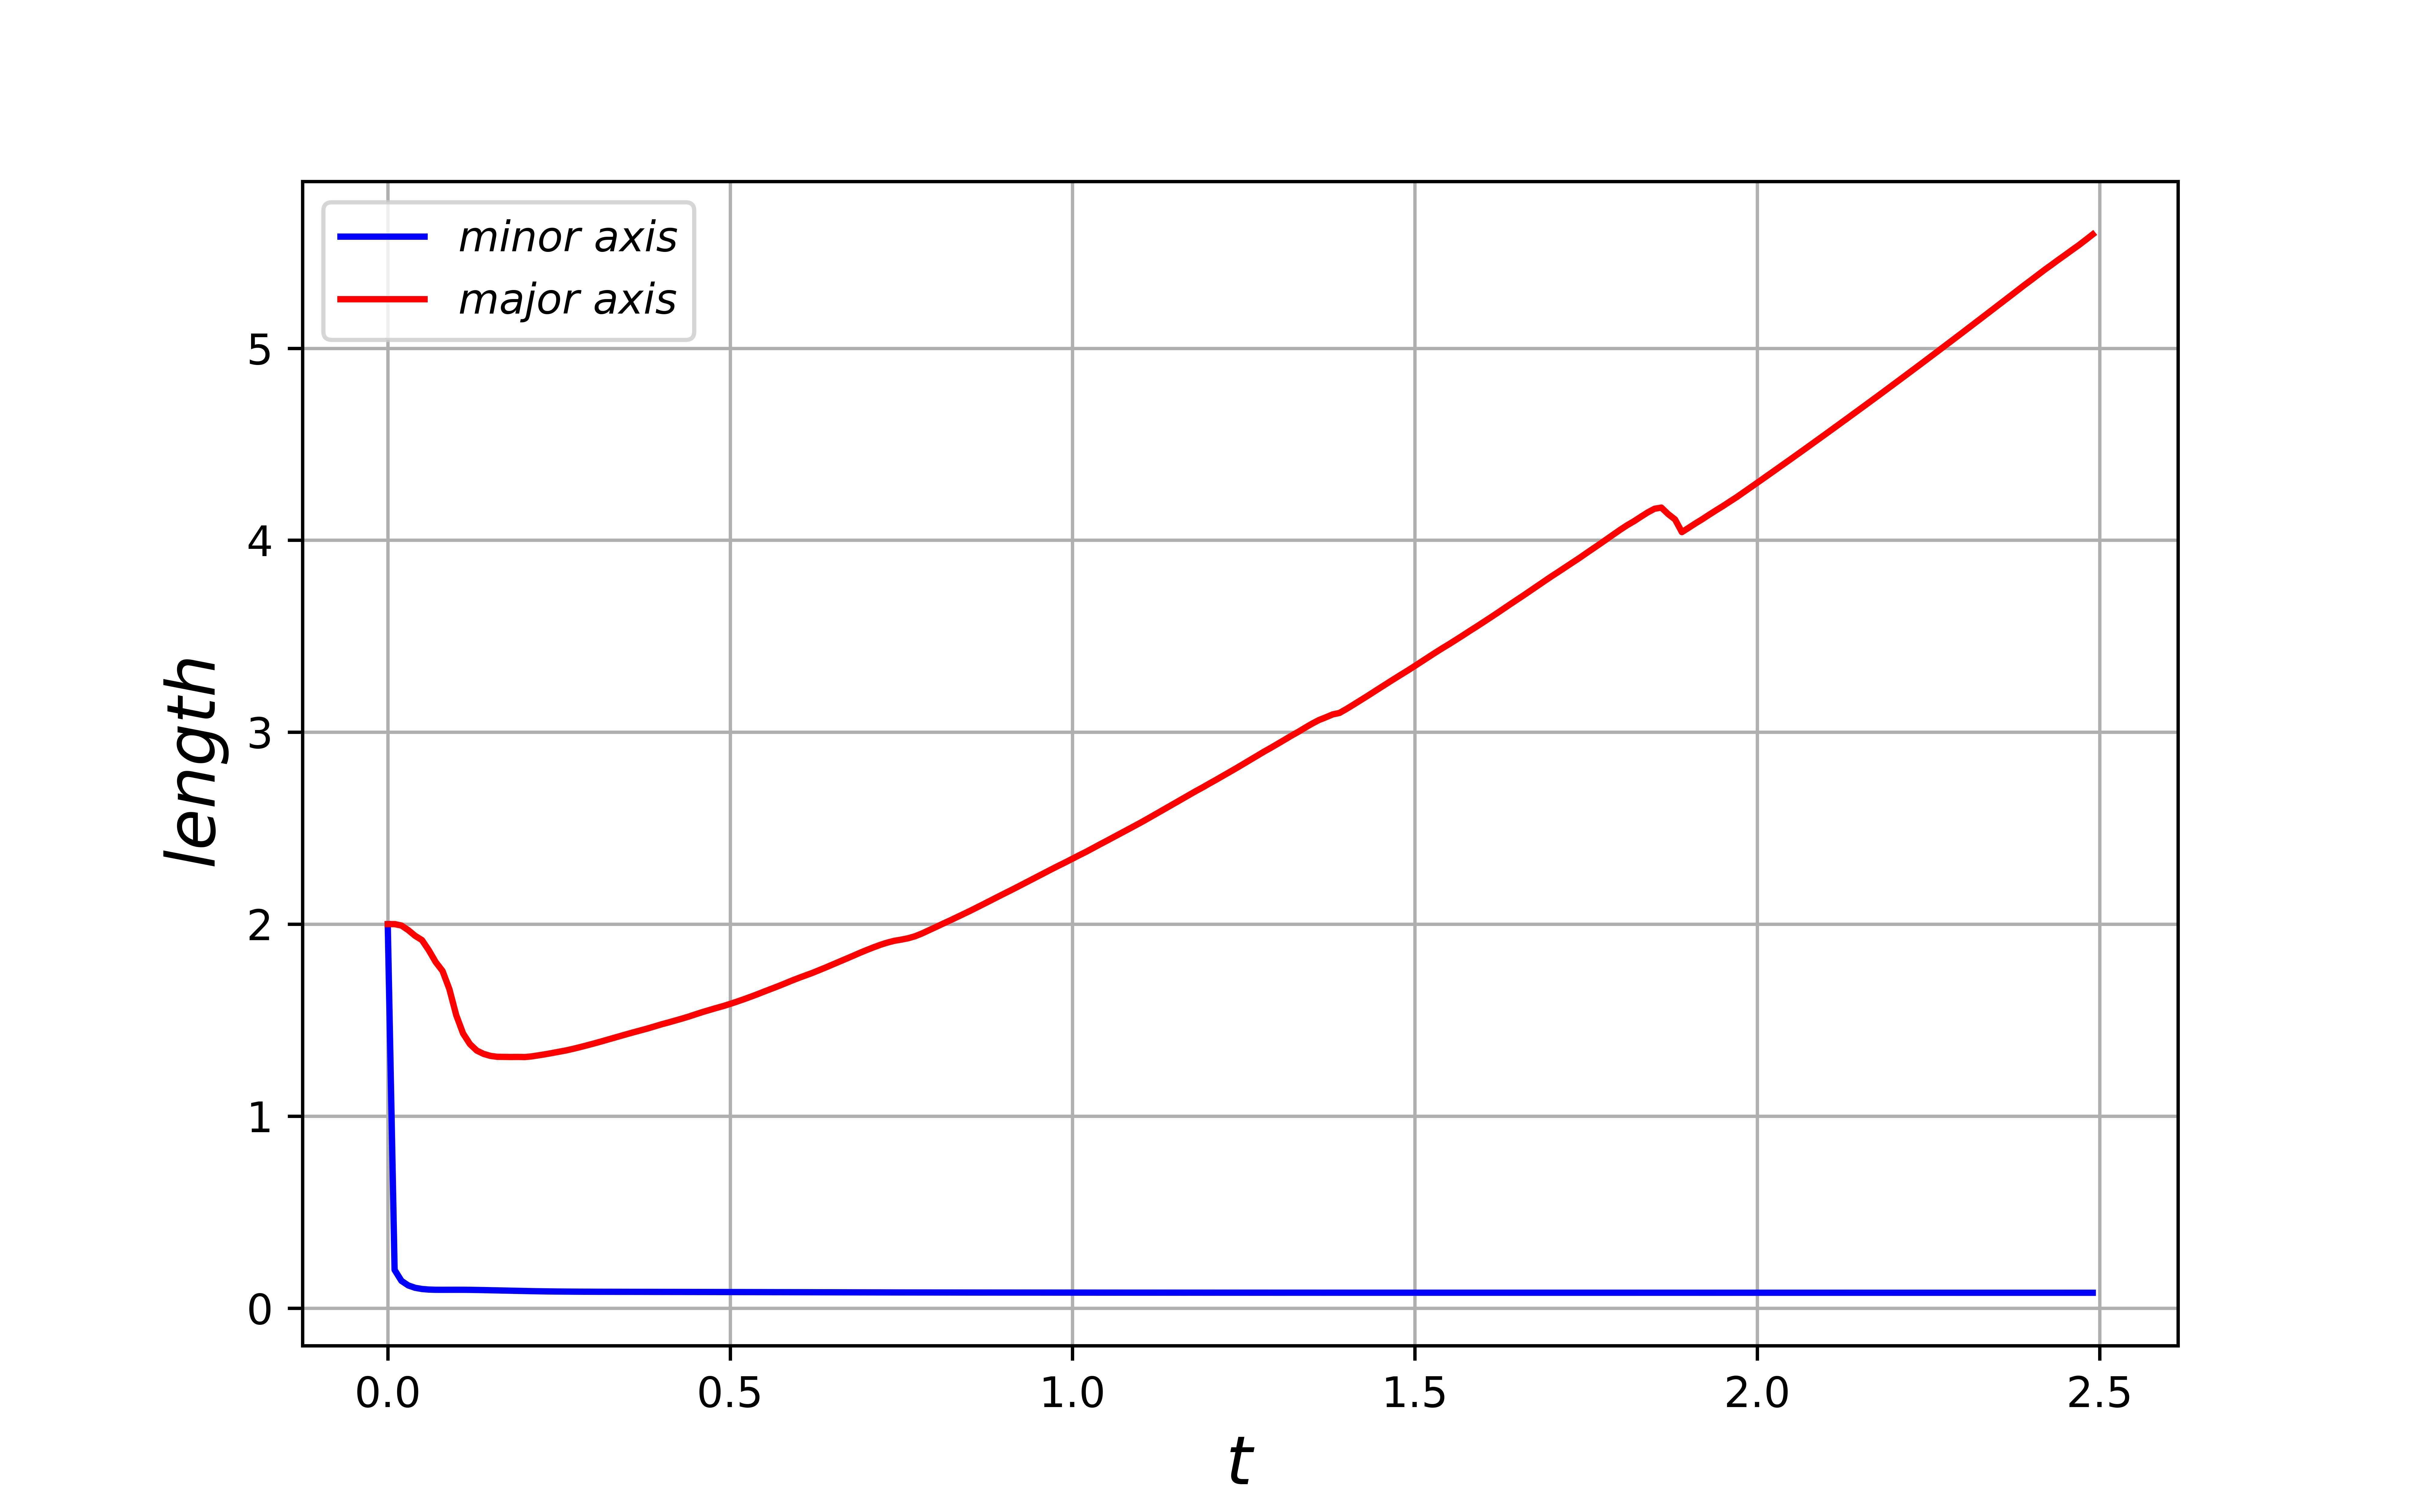
\includegraphics[width=\linewidth]{plots/part2-f-1-axes.png}
        \caption*{Major and Minor Axes}
    \end{minipage}

    \caption{Base-Station $B_2(-32, -50)$}
\end{figure}


\begin{figure}[H]
    \centering
    \begin{minipage}{0.49\linewidth}
        \centering
        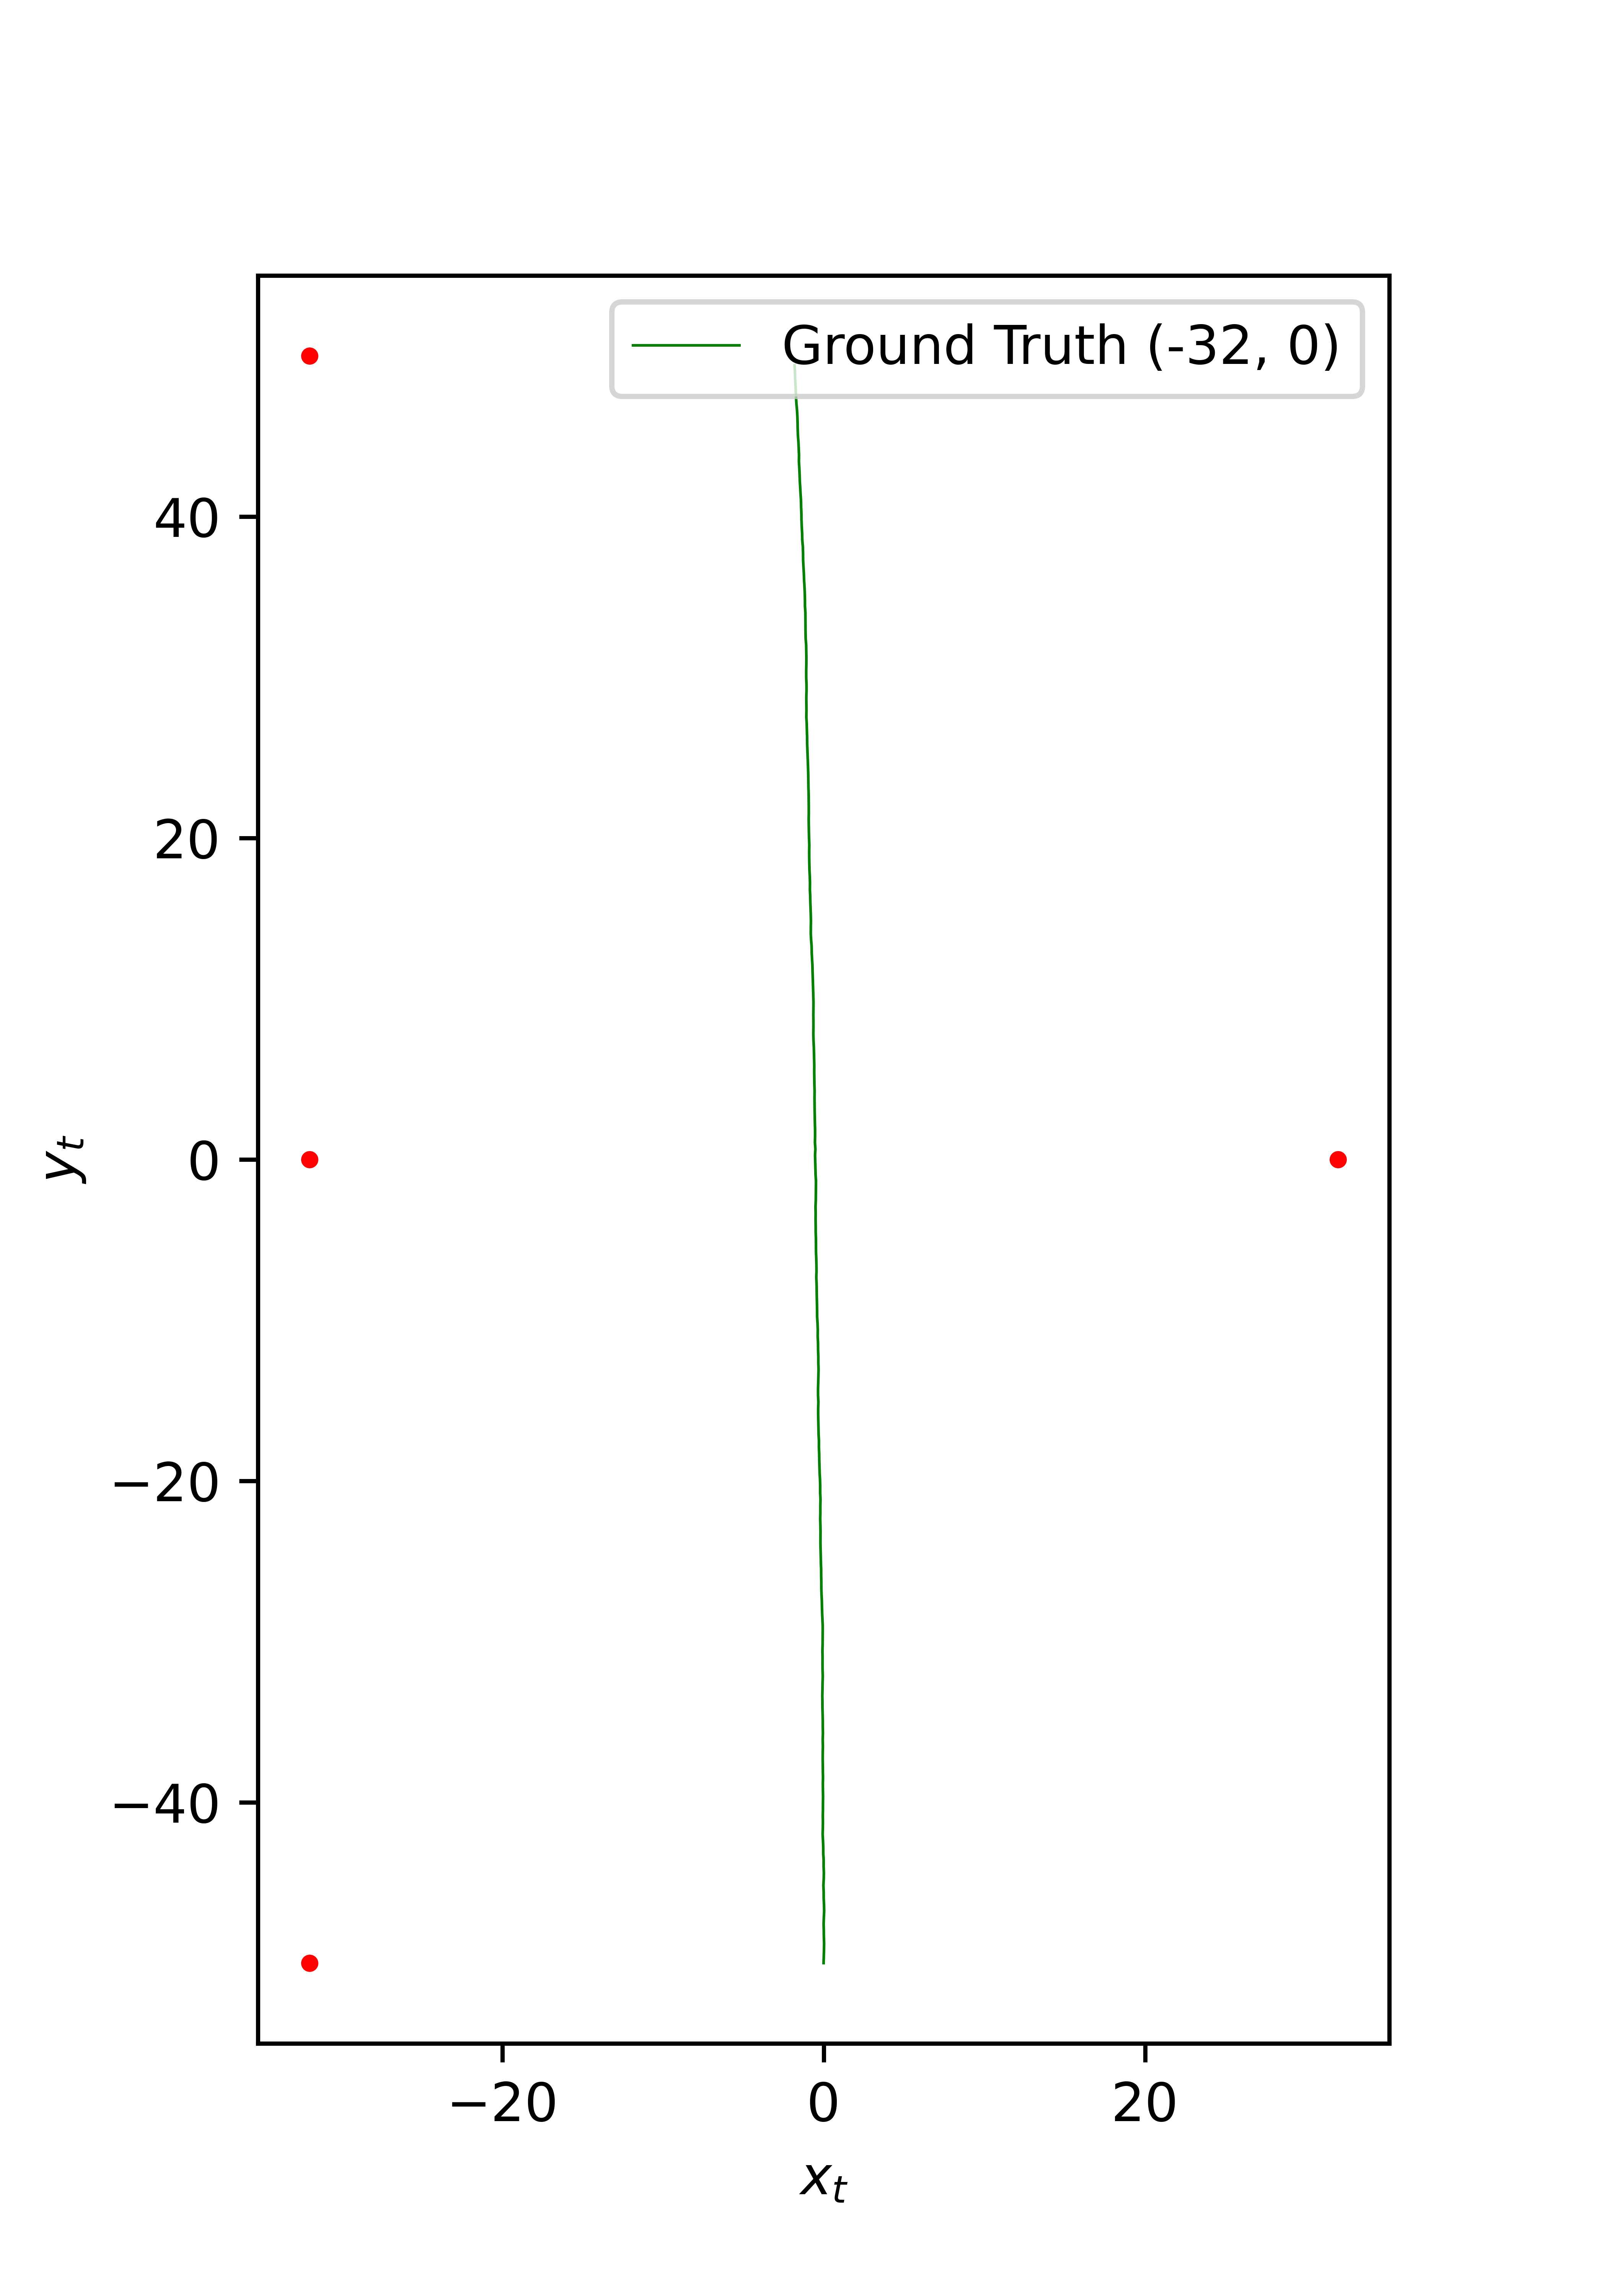
\includegraphics[width=\linewidth]{plots/part2-f-2-GT.png}
        \caption*{Ground Truth}
    \end{minipage}
    \hfill
    \begin{minipage}{0.49\linewidth}
        \centering
        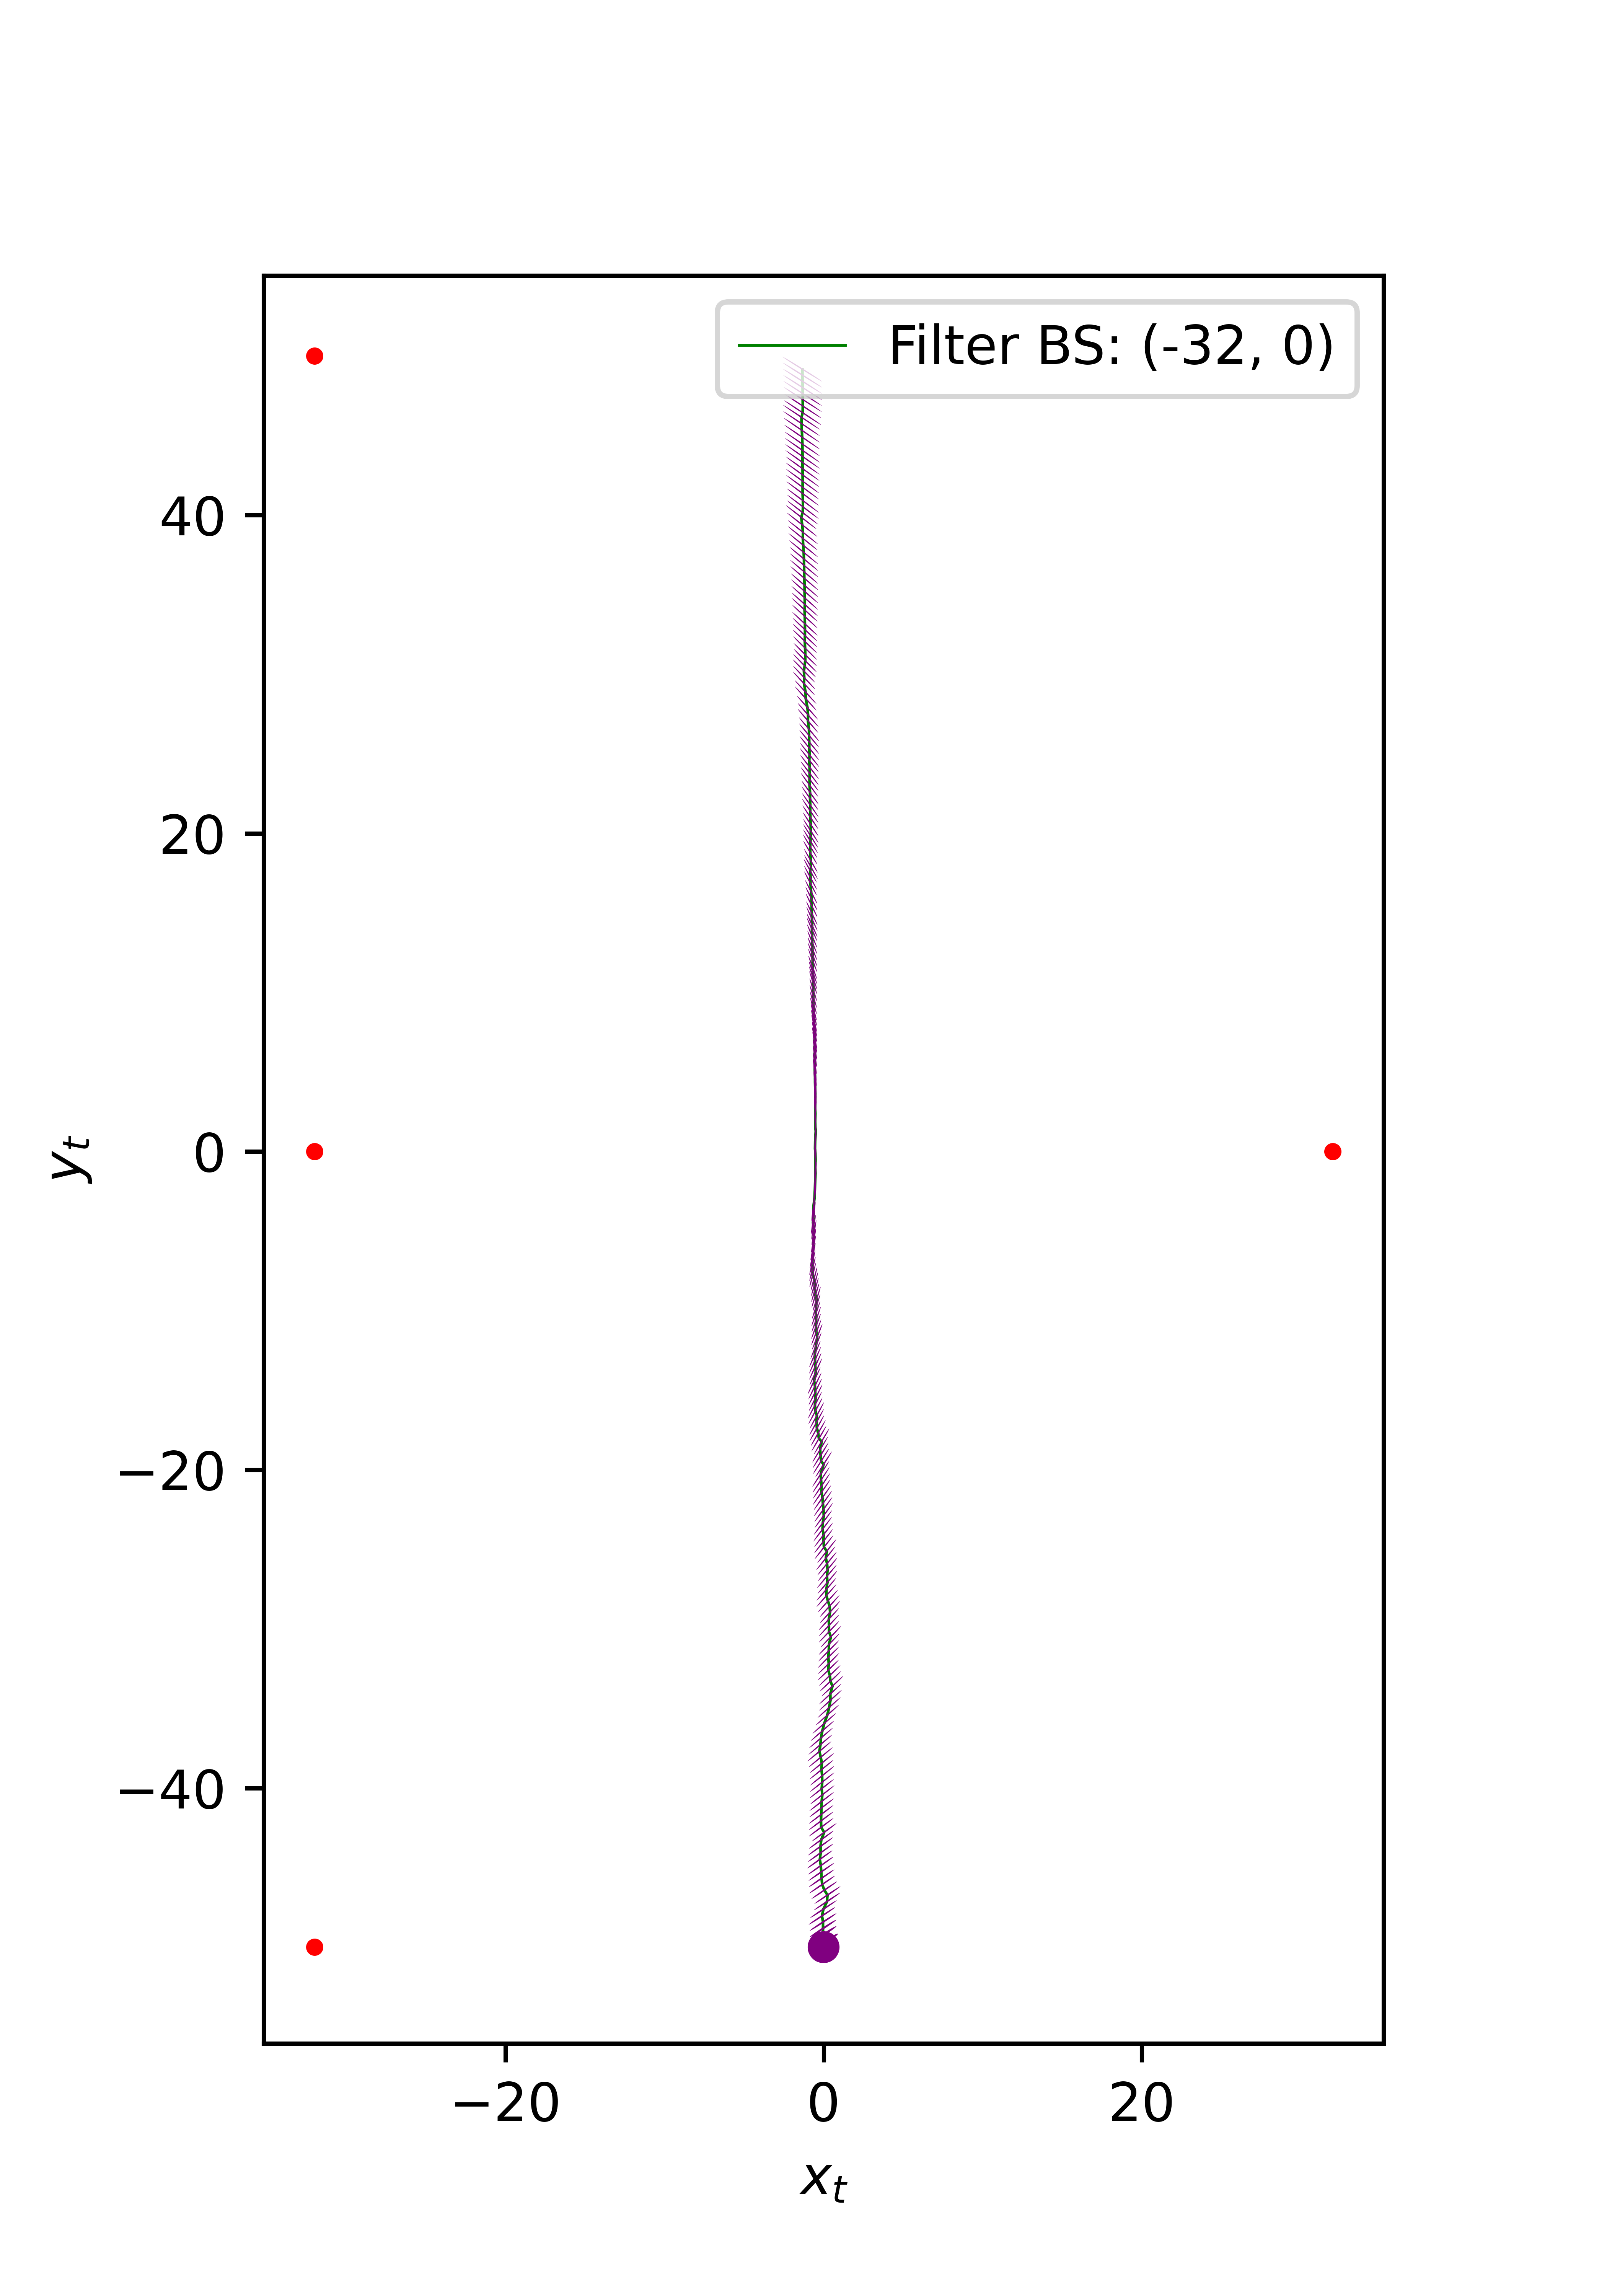
\includegraphics[width=\linewidth]{plots/part2-f-2-filter.png}
        \caption*{Kalman Filter}
    \end{minipage}
    \vspace{-0.1cm}
    \begin{minipage}{\linewidth}
        \centering
        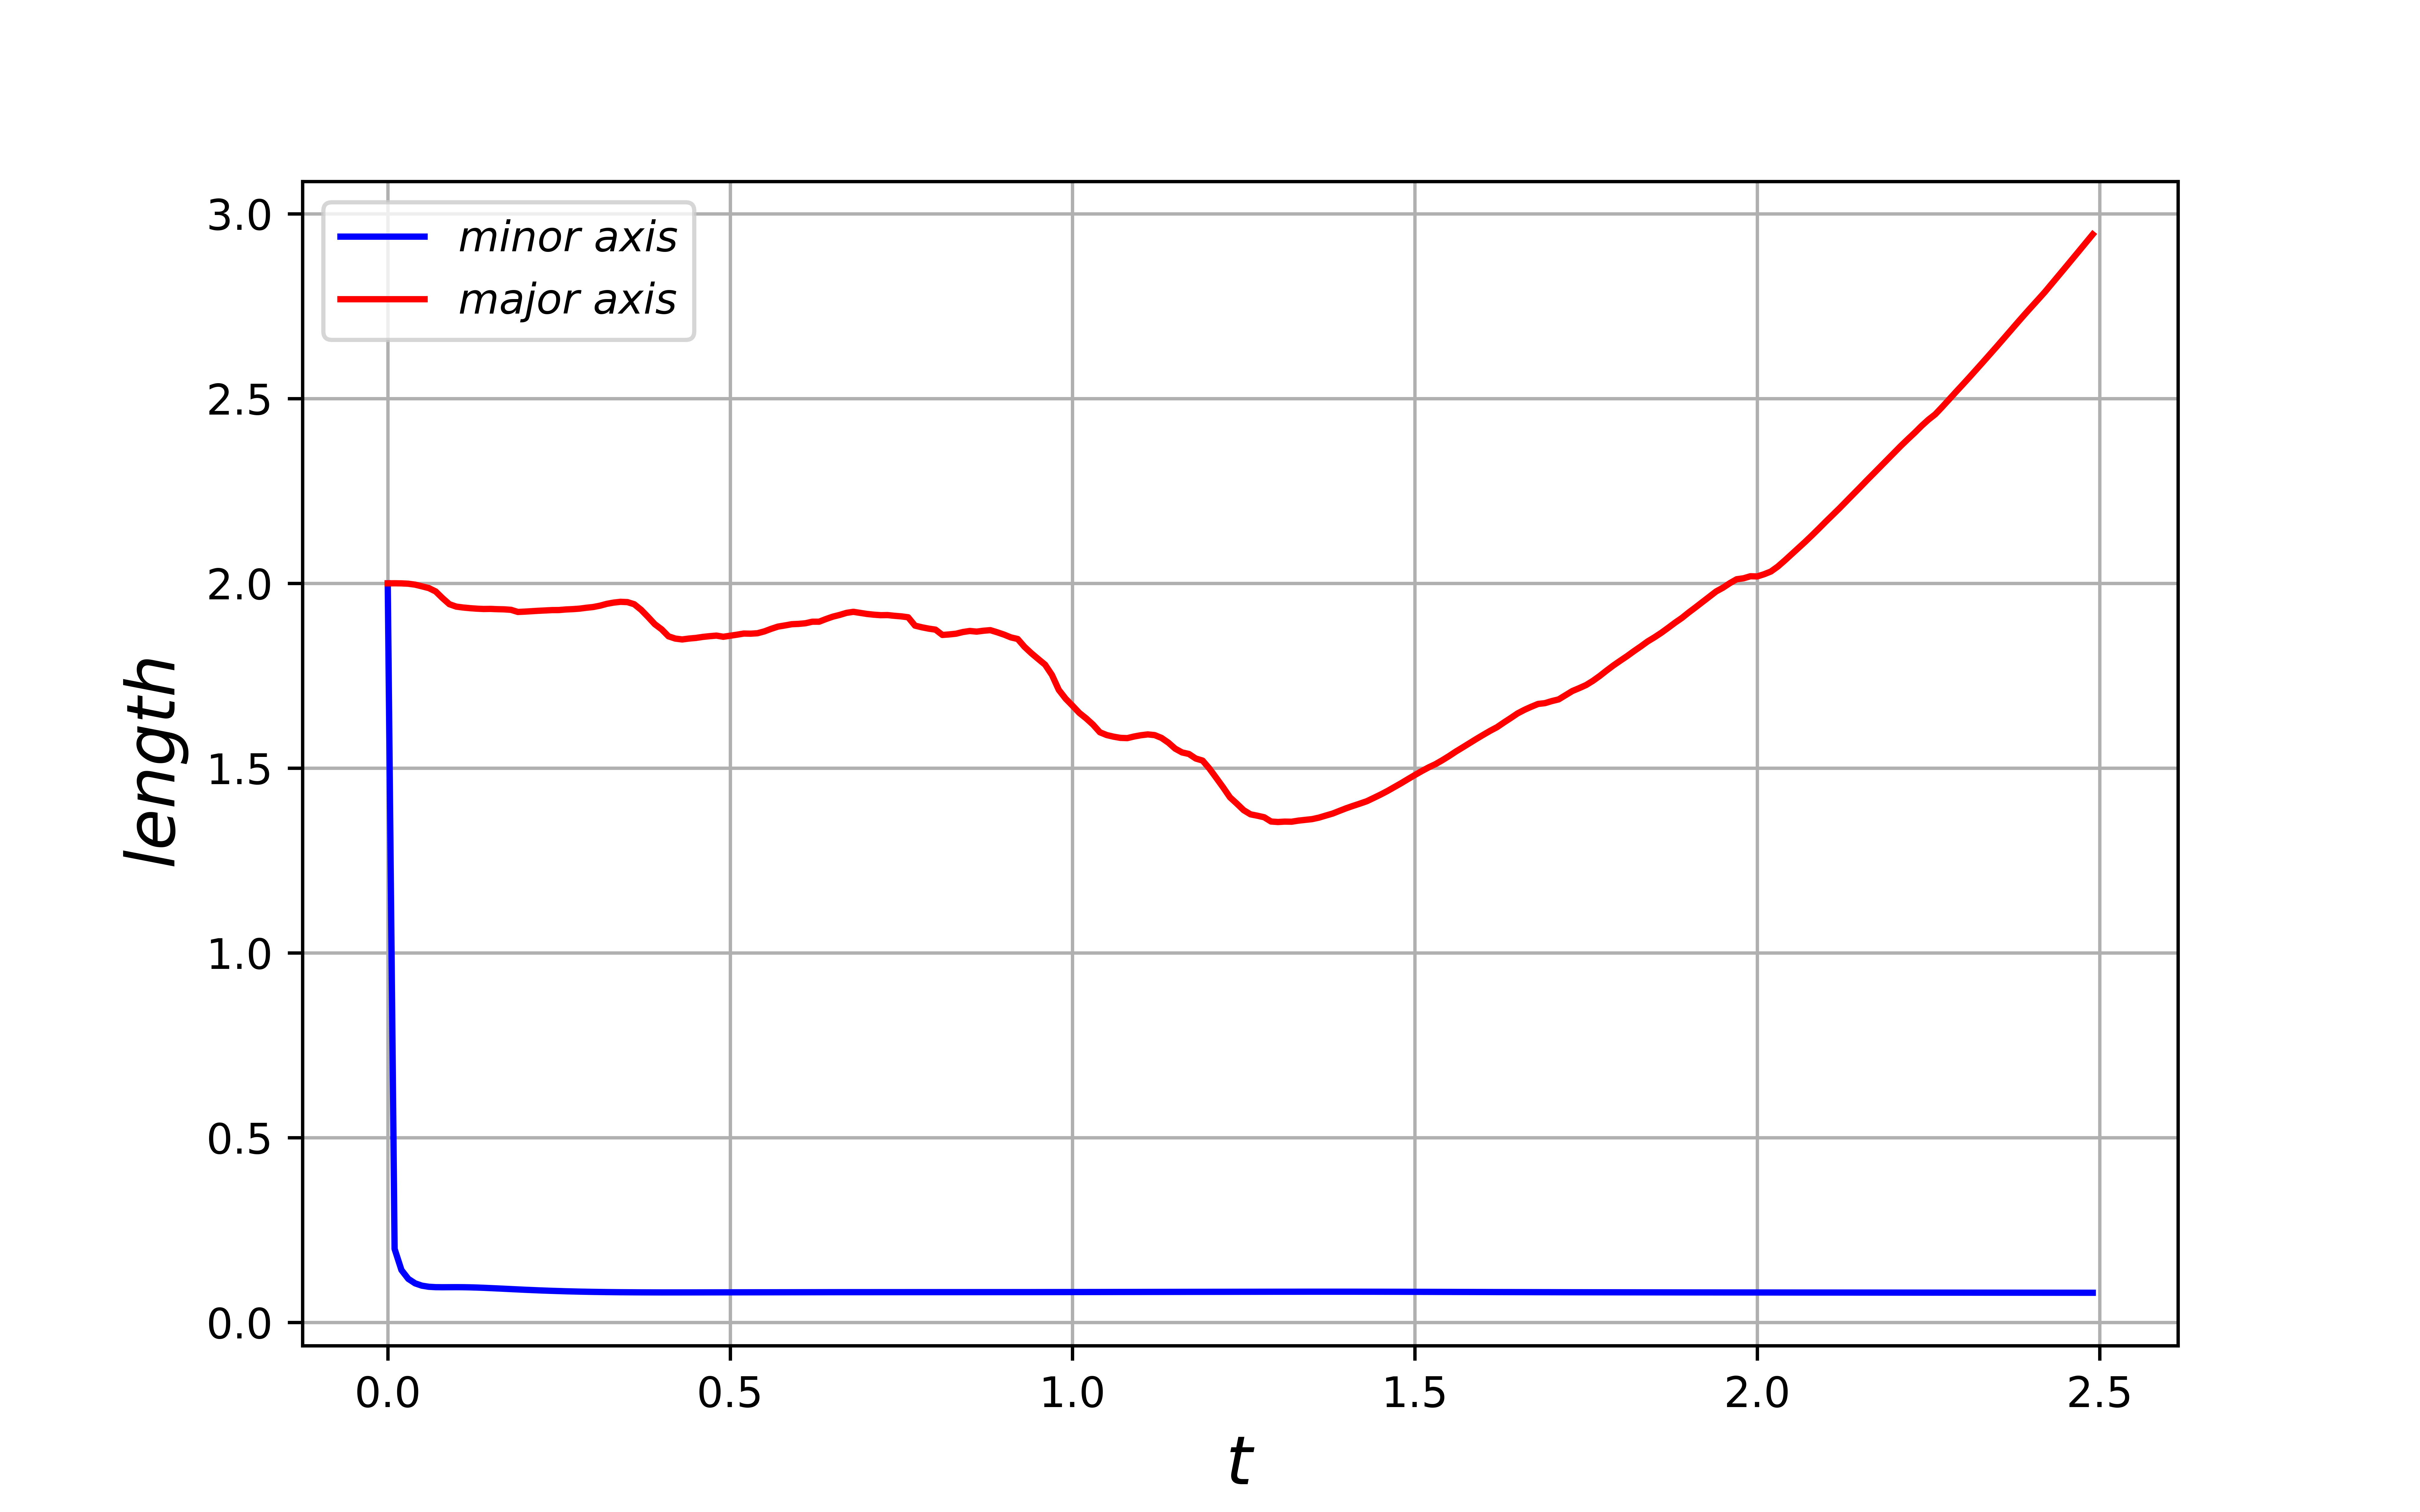
\includegraphics[width=\linewidth]{plots/part2-f-2-axes.png}
        \caption*{Major and Minor Axes}
    \end{minipage}
    \caption{Base-Station $B_3(-32, 0)$}
    \label{fig:part2fB3-uncertainty_ellipse}
\end{figure}


\begin{figure}[H]
    \centering
    \begin{minipage}{0.49\linewidth}
        \centering
        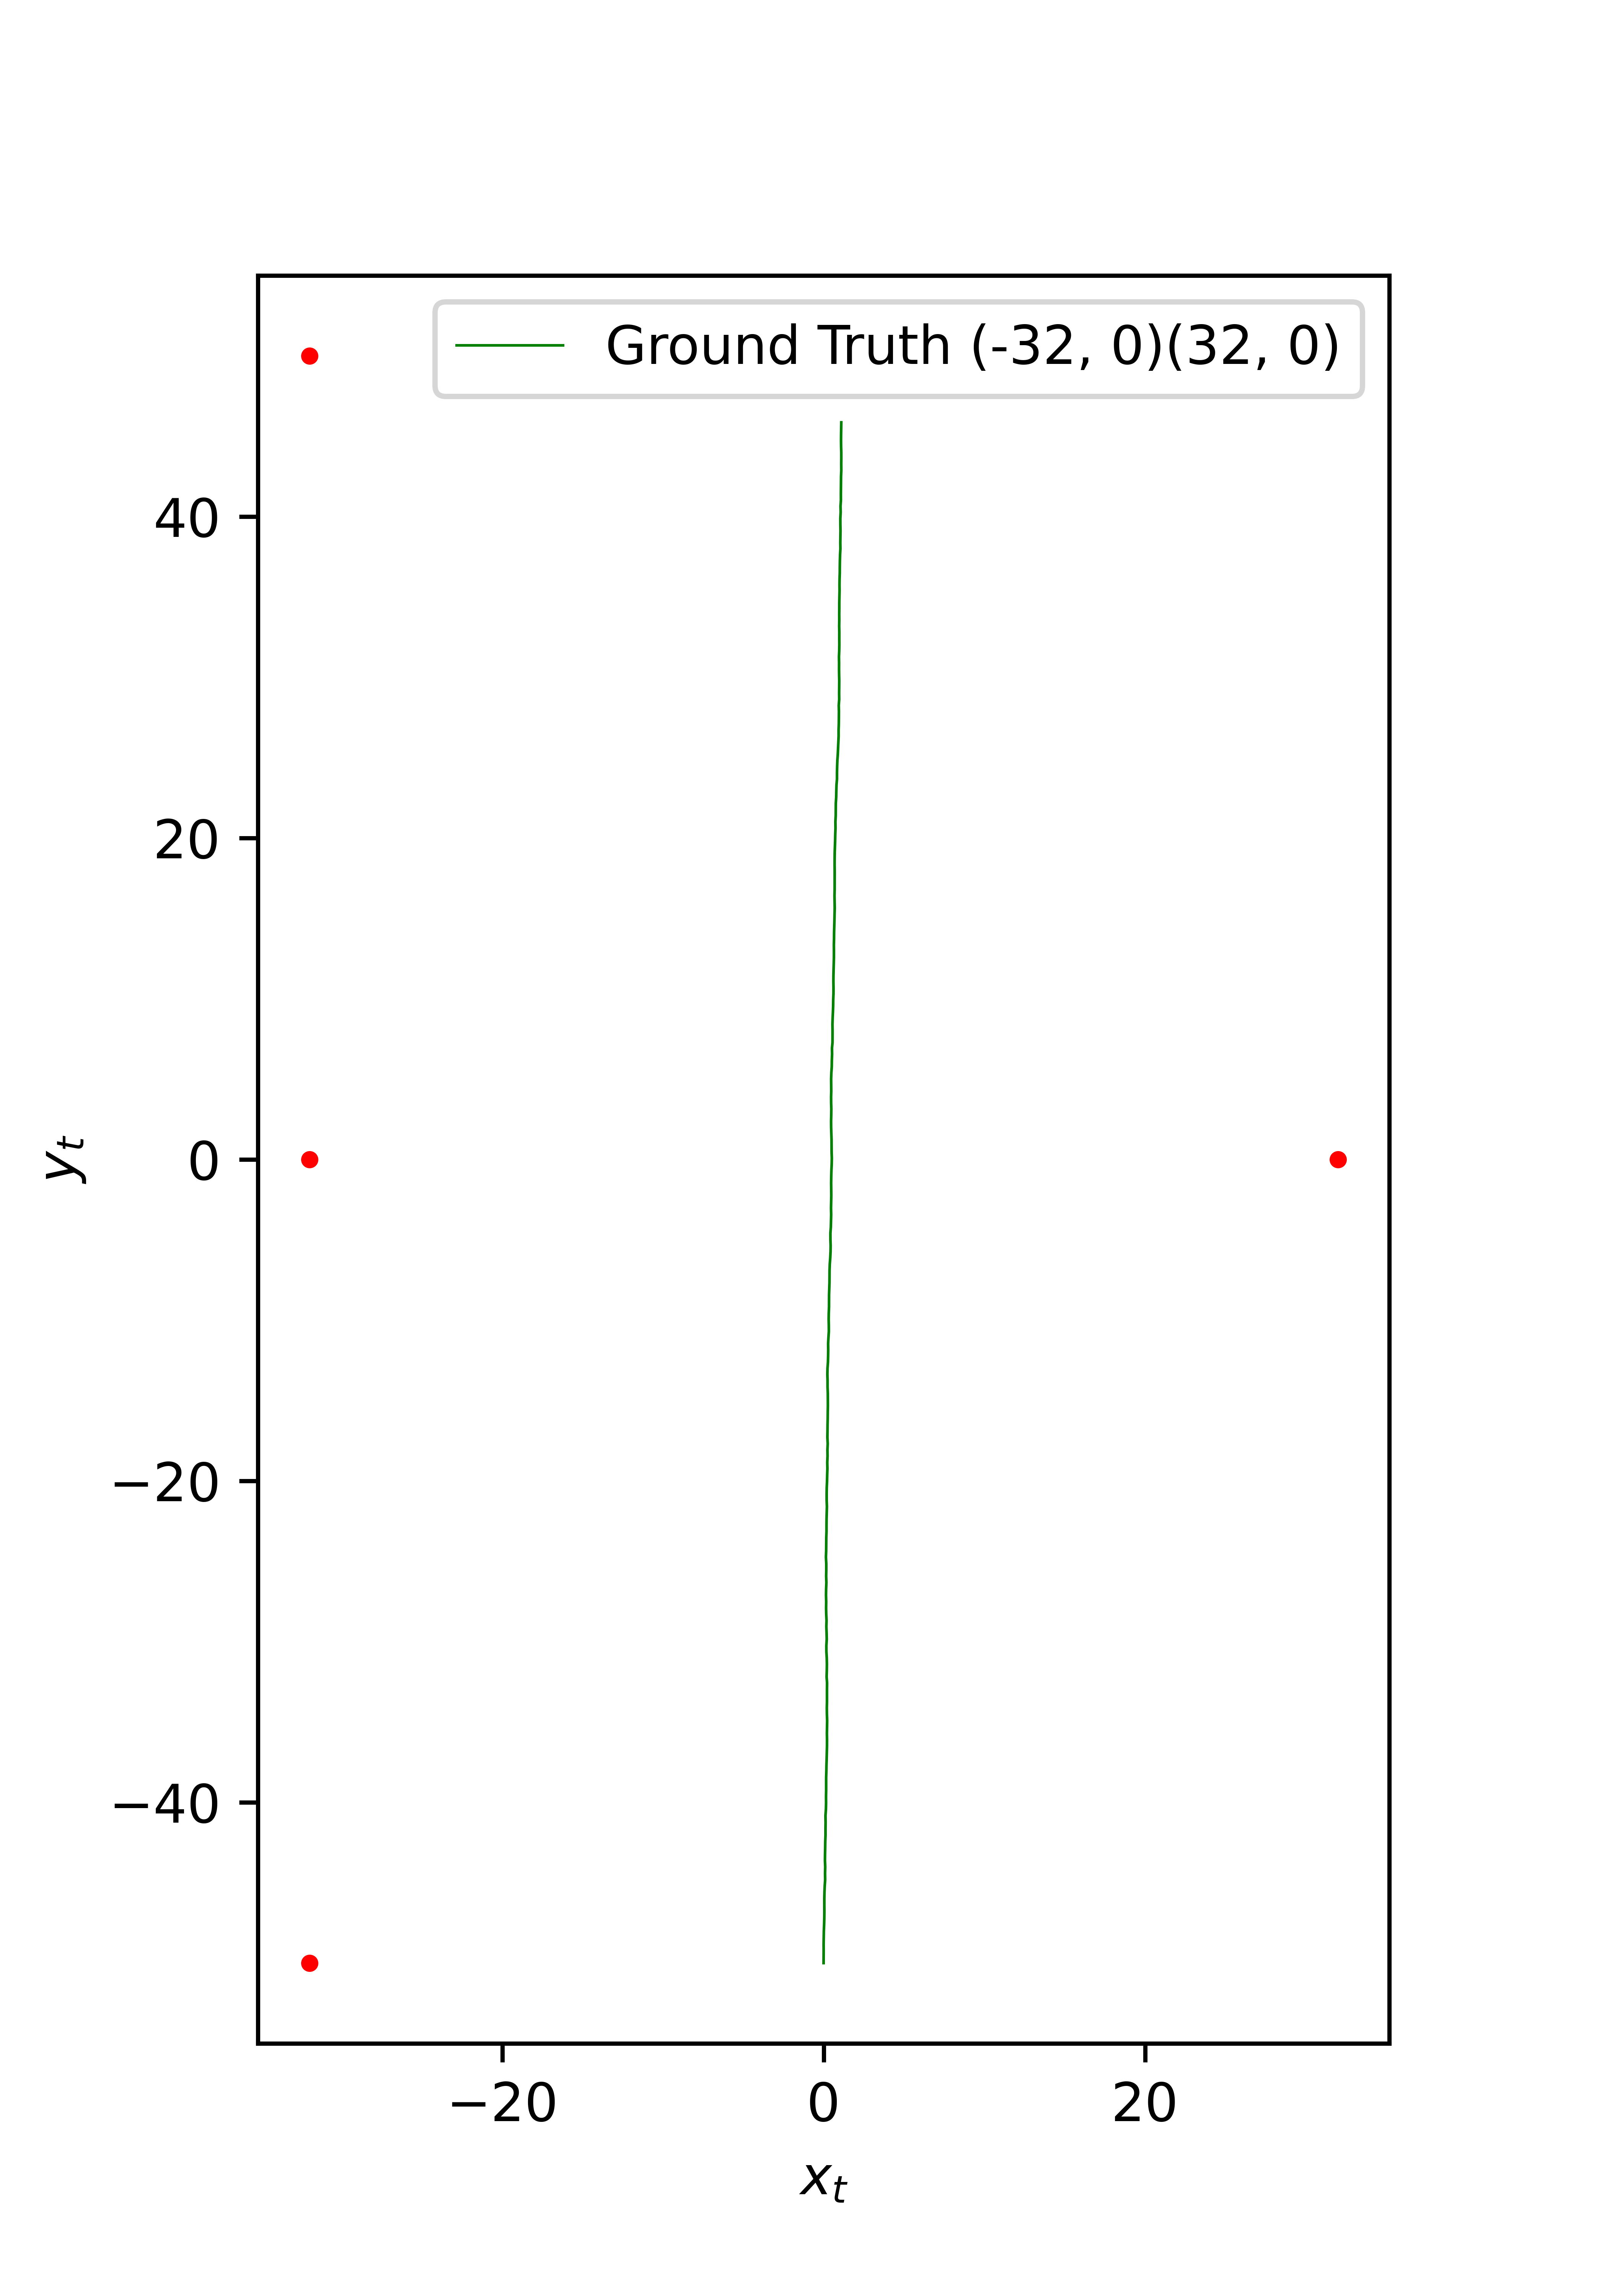
\includegraphics[width=\linewidth]{plots/part2-f-3-GT.png}
        \caption*{Ground Truth}
    \end{minipage}
    \hfill
    \begin{minipage}{0.49\linewidth}
        \centering
        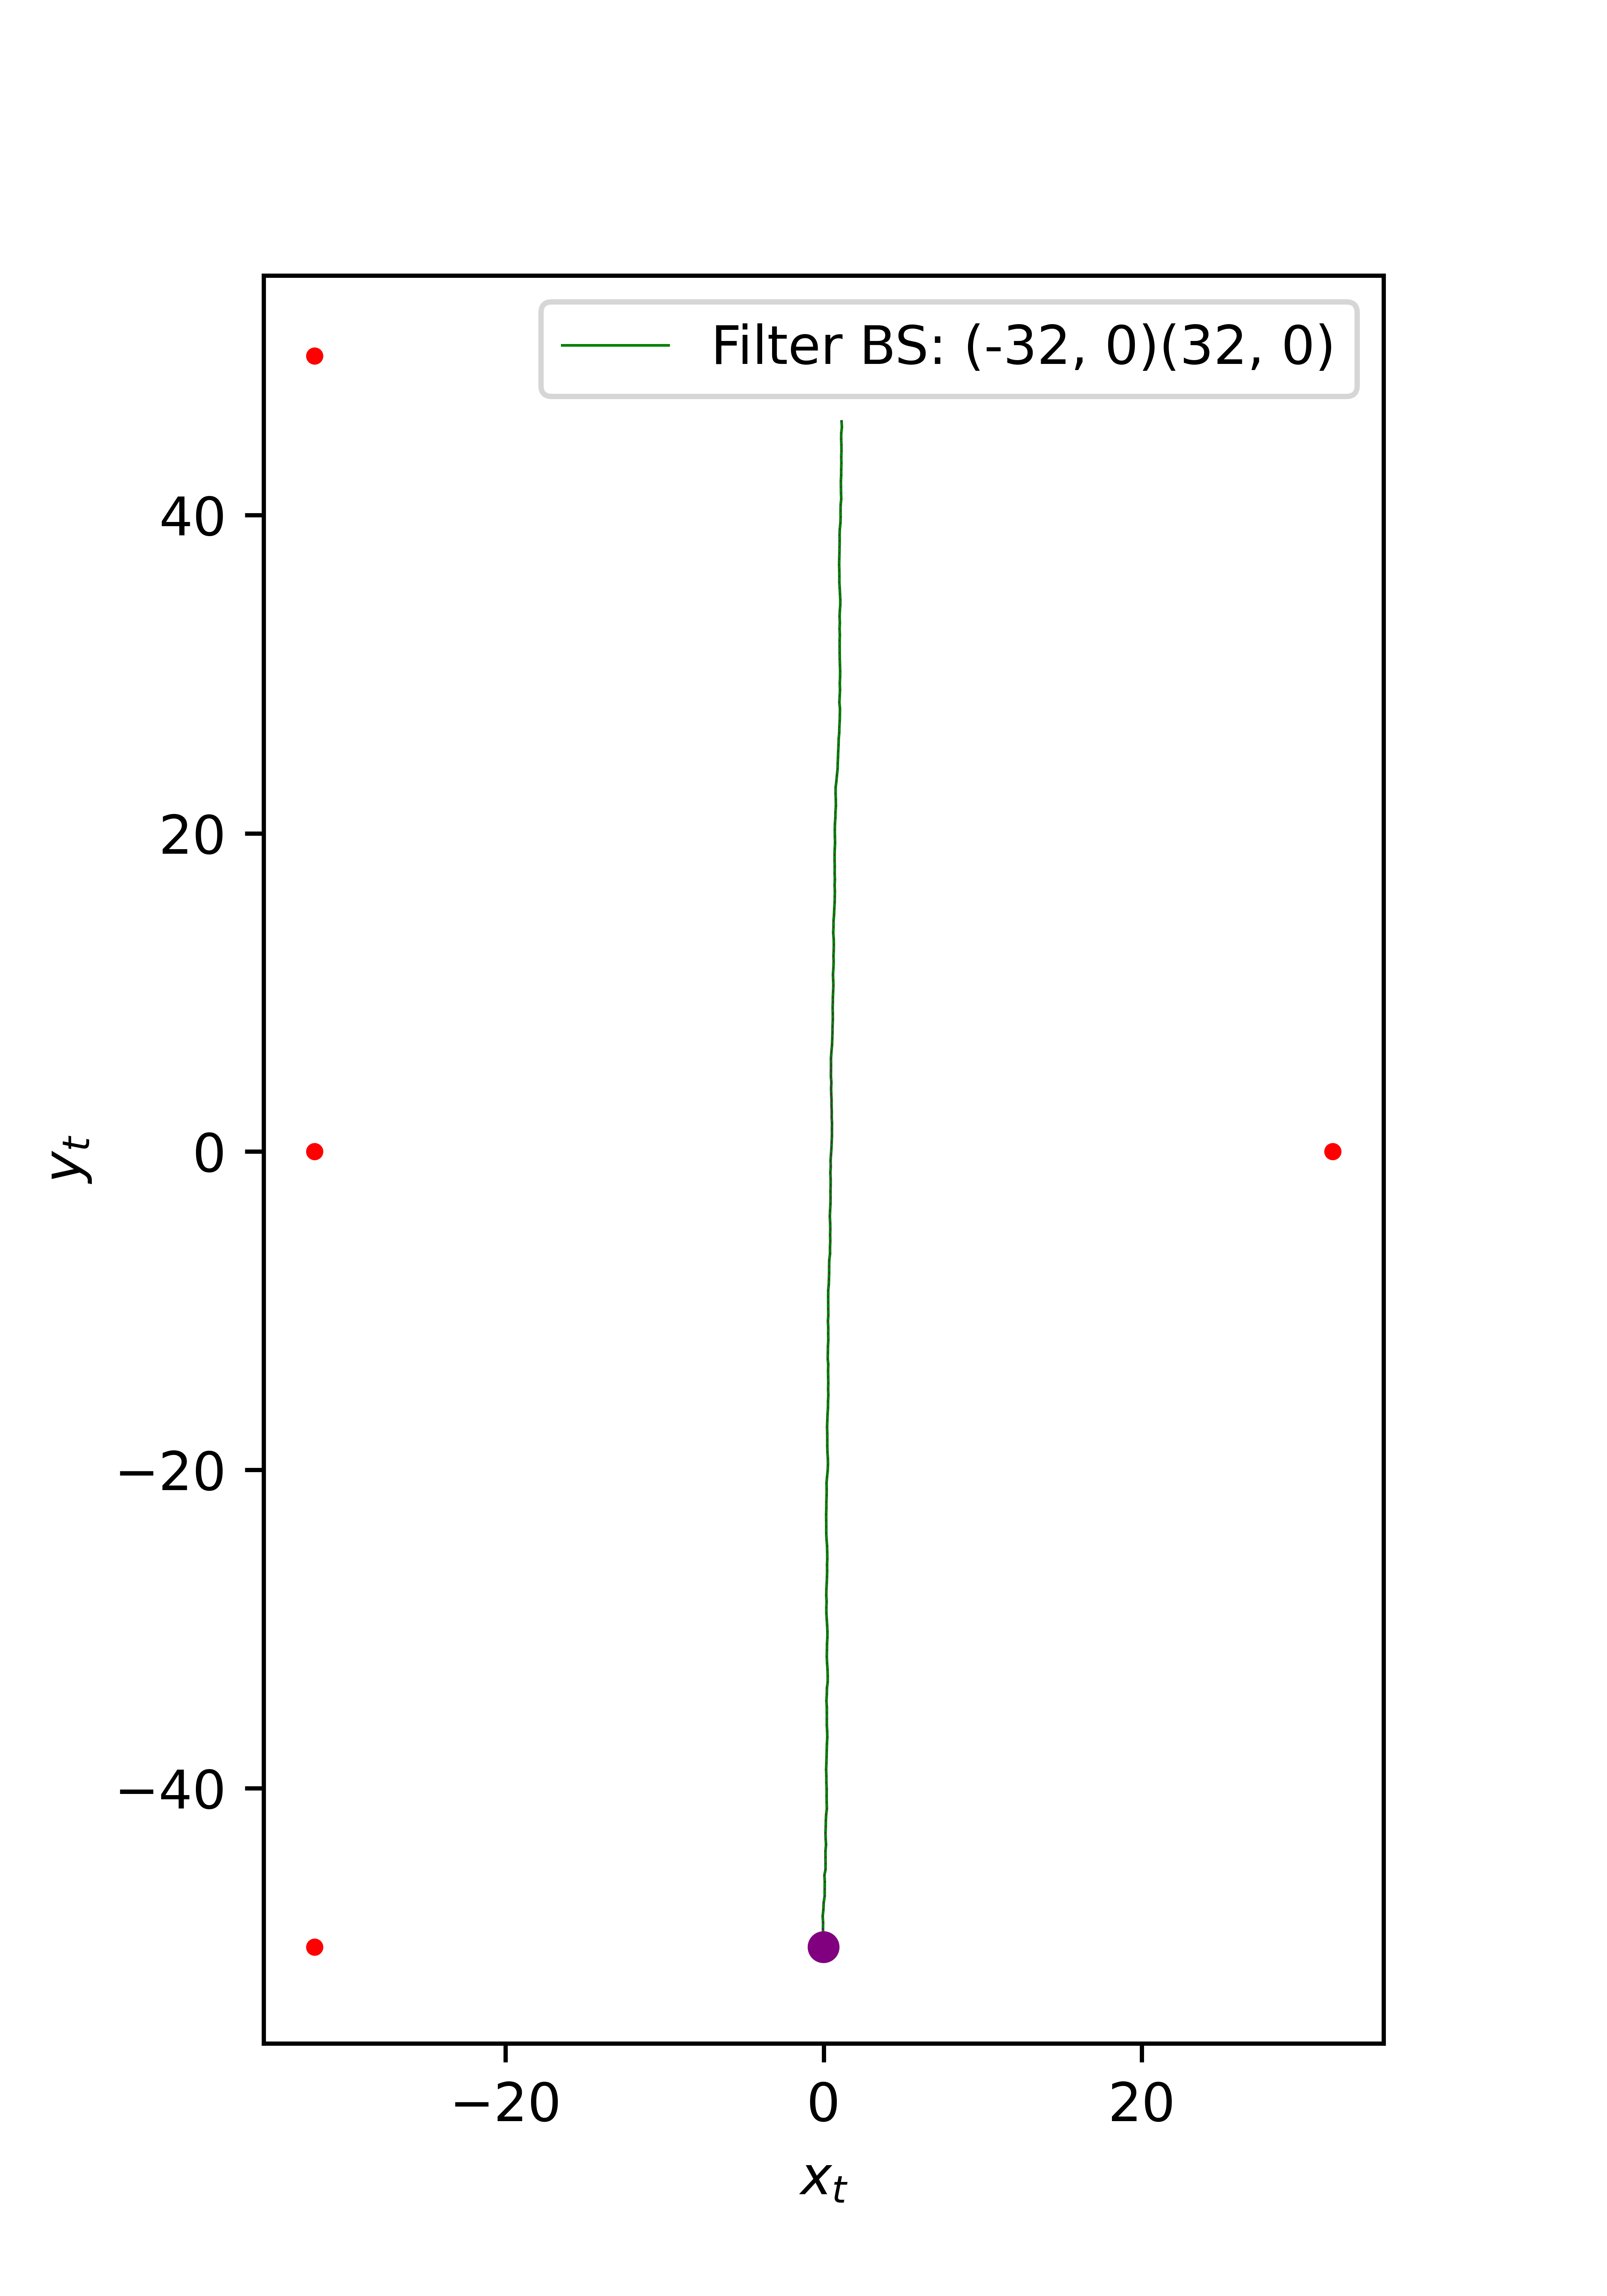
\includegraphics[width=\linewidth]{plots/part2-f-3-filter.png}
        \caption*{Kalman Filter}
    \end{minipage}
    \vspace{-0.1cm}
    \begin{minipage}{\linewidth}
        \centering
        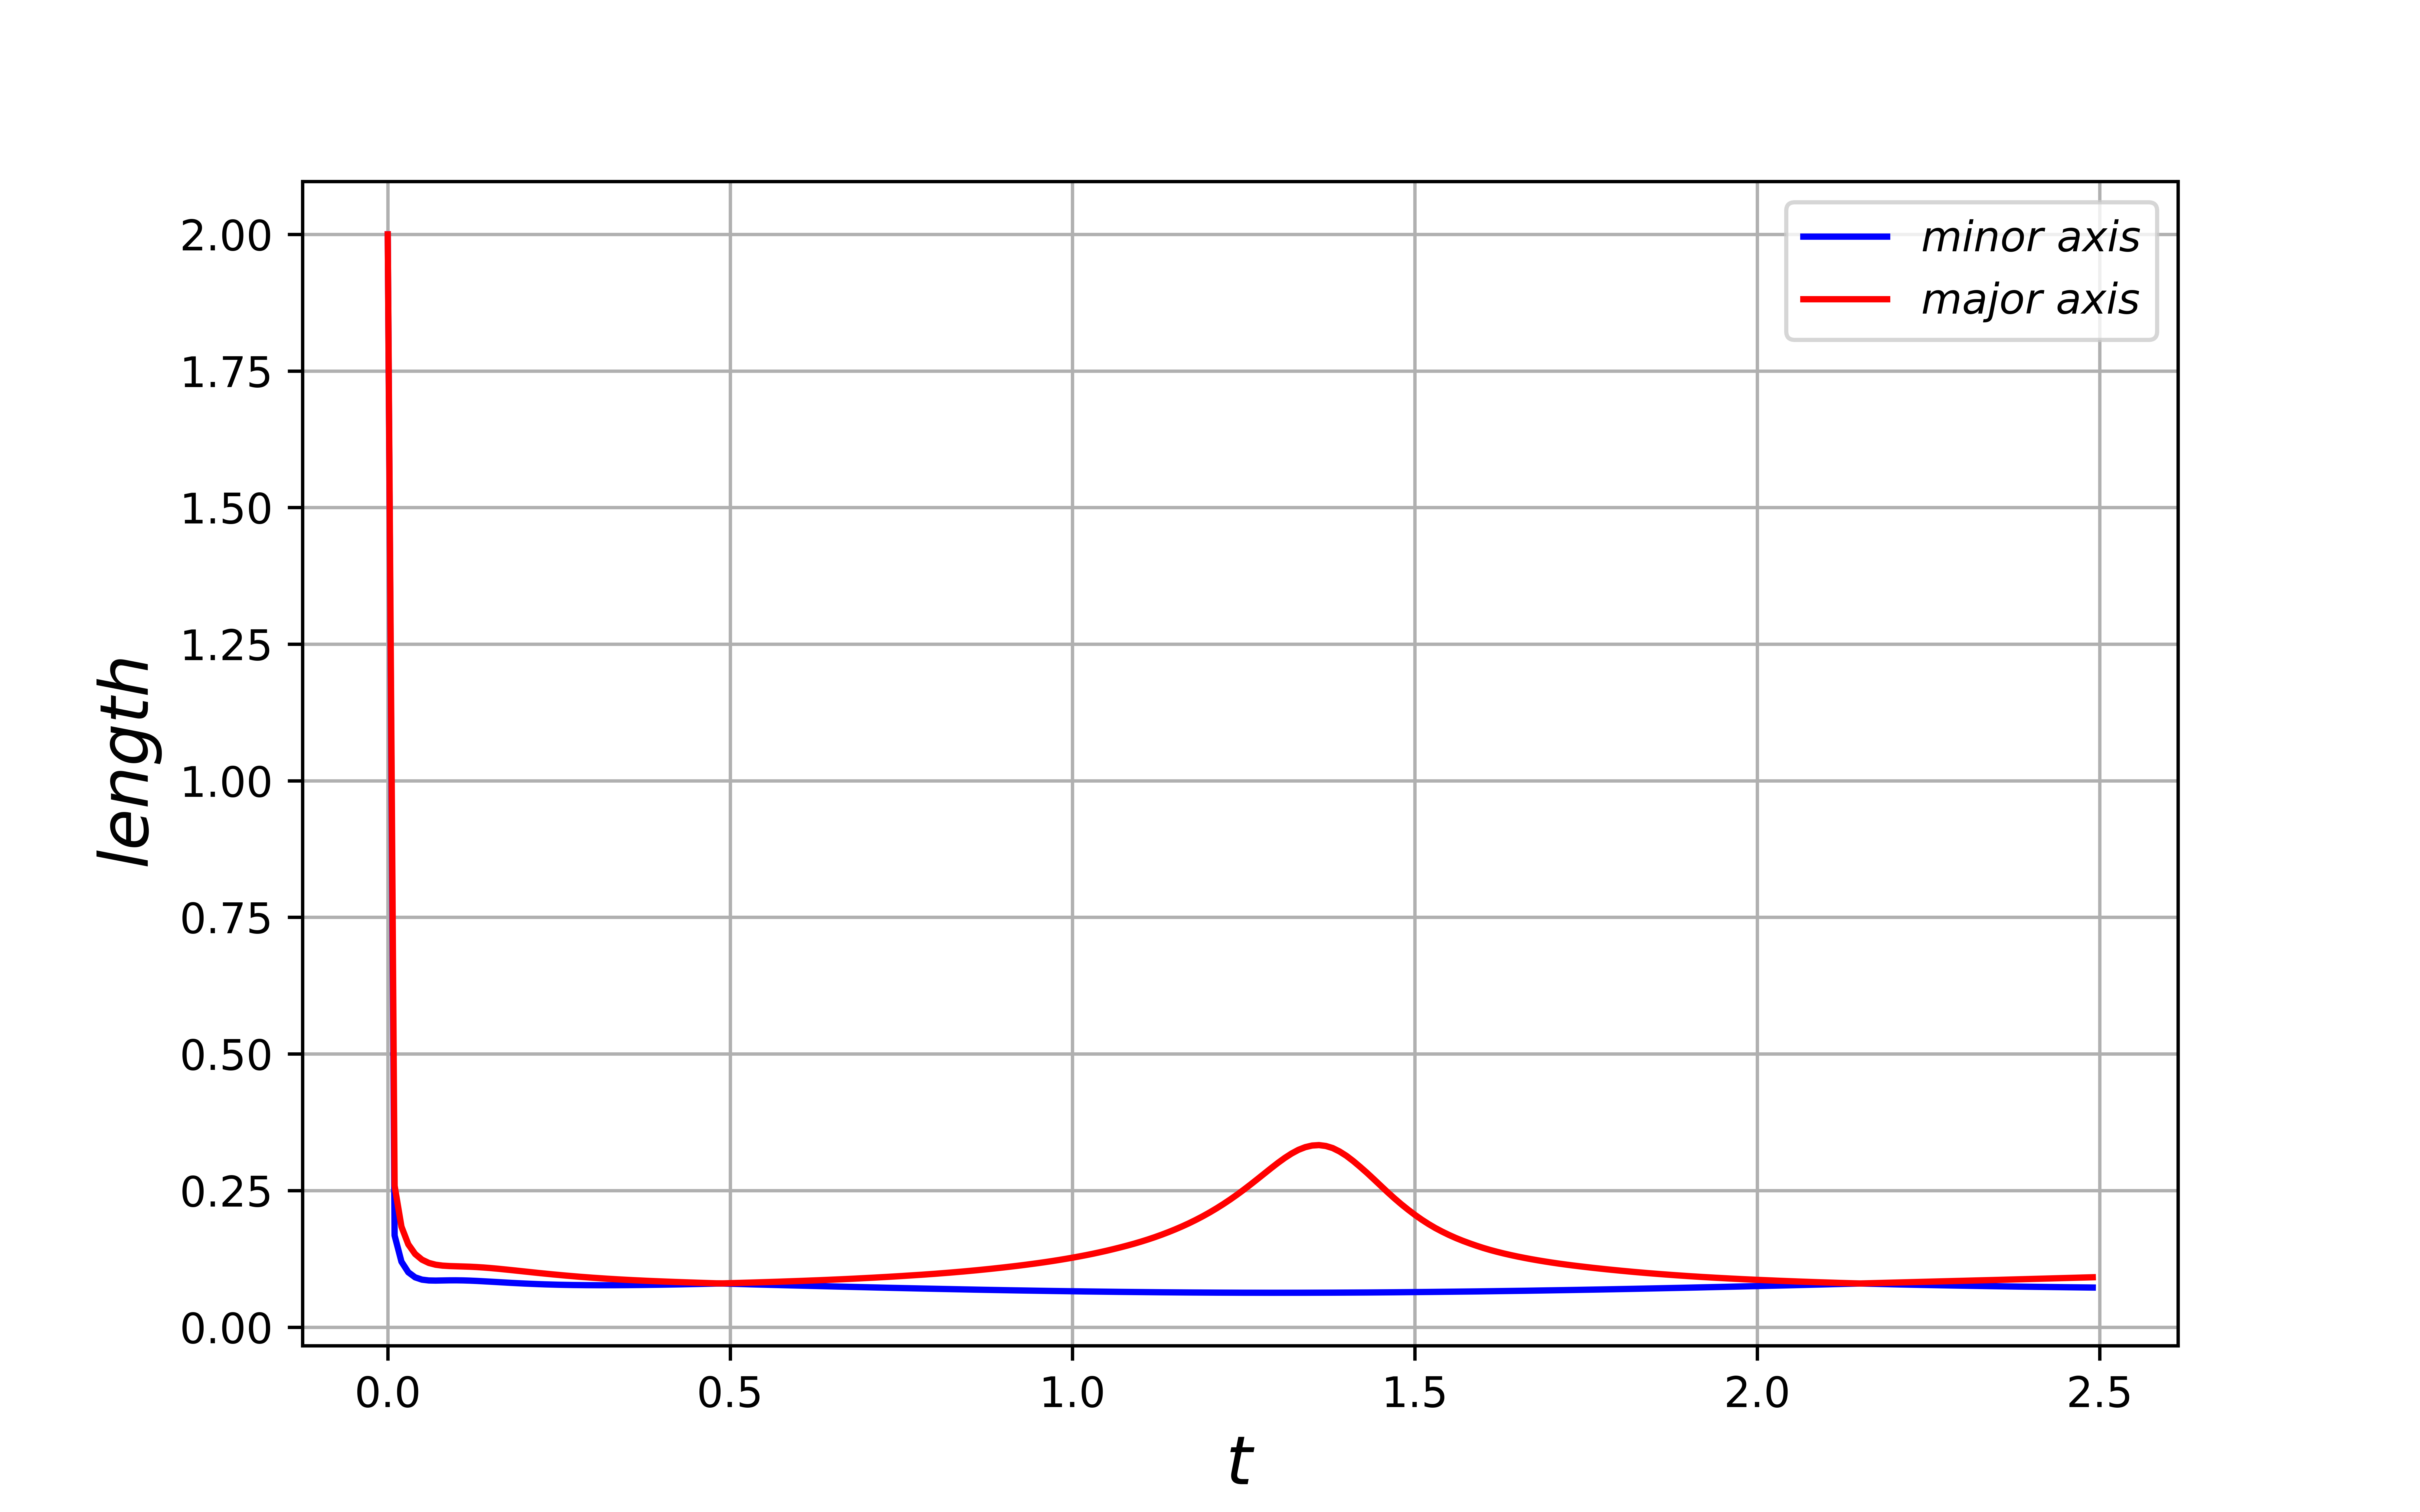
\includegraphics[width=\linewidth]{plots/part2-f-3-axes.png}
        \caption*{Major and Minor Axes}
    \end{minipage}

    \caption{Base-Station $B_3(-32, 0), B_4 (32, 0)$}
\end{figure}
